% ======================================================================
% main.tex  –  Quantum Error Correction Lecture Notes  v3.0
% Extended edition with additional examples, worked calculations,
% intuitive explanations, and TikZ visual aids.
% Designed for undergraduate students with basic linear algebra and
% introductory quantum mechanics background.
% ======================================================================

\documentclass[11pt, a4paper]{article}

% ======================================================================
% PACKAGES
% ======================================================================
\usepackage[utf8]{inputenc}
\usepackage[T1]{fontenc}
\usepackage{amsmath, amssymb, amsthm}
\usepackage{bm}
\usepackage{graphicx}
\usepackage[margin=1in]{geometry}
\usepackage{xcolor}
\usepackage[colorlinks=true, linkcolor=blue, citecolor=cyan,
            urlcolor=magenta,
            pdftitle={Quantum Error Correction Lecture Notes v3.0},
            pdfauthor={Quantum Computing Course},
            pdfpagemode=UseOutlines, bookmarks=true]{hyperref}
\usepackage{braket}
\usepackage{tikz}
\usetikzlibrary{quantikz, positioning, shapes.geometric, arrows.meta,
                matrix, decorations.pathreplacing, fit, calc, backgrounds}
\usepackage{enumitem}
\usepackage{tcolorbox}
\tcbuselibrary{skins, breakable, theorems}
\usepackage{booktabs}
\usepackage{array}
\usepackage{multirow}
\usepackage{mdframed}
\usepackage{cancel}
\usepackage{mathtools}
\usepackage{float}

% ======================================================================
% COLOURS
% ======================================================================
\definecolor{keyblue}{RGB}{0,102,204}
\definecolor{warncolor}{RGB}{180,80,0}
\definecolor{examplegreen}{RGB}{0,120,60}
\definecolor{defcolor}{RGB}{80,0,120}
\definecolor{lightblue}{RGB}{230,242,255}
\definecolor{lightyellow}{RGB}{255,252,230}
\definecolor{lightgreen}{RGB}{230,255,240}
\definecolor{lightpurple}{RGB}{245,230,255}
\definecolor{lightred}{RGB}{255,235,235}
\definecolor{lightgray}{RGB}{245,245,245}
\definecolor{darkgray}{RGB}{60,60,60}
\definecolor{teal}{RGB}{0,128,128}
\definecolor{lightteal}{RGB}{230,248,248}

% ======================================================================
% TCOLORBOX ENVIRONMENTS
% ======================================================================

% Key Point box (blue)
\newtcolorbox{keypoint}{
  enhanced, breakable,
  colback=lightblue, colframe=keyblue,
  fonttitle=\bfseries, title={Key Point},
  left=6pt, right=6pt, top=4pt, bottom=4pt,
  arc=4pt
}

% Caution / Warning box (orange)
\newtcolorbox{caution}{
  enhanced, breakable,
  colback=lightyellow, colframe=warncolor,
  fonttitle=\bfseries, title={Caution},
  left=6pt, right=6pt, top=4pt, bottom=4pt,
  arc=4pt
}

% Worked Example box (green)
\newtcolorbox[auto counter, number within=section]{workedexample}[1][]{
  enhanced, breakable,
  colback=lightgreen, colframe=examplegreen,
  fonttitle=\bfseries,
  title={Worked Example \thetcbcounter\ifstrempty{#1}{}{: #1}},
  left=6pt, right=6pt, top=4pt, bottom=4pt,
  arc=4pt
}

% Intuition box (teal)
\newtcolorbox{intuition}{
  enhanced, breakable,
  colback=lightteal, colframe=teal,
  fonttitle=\bfseries, title={Intuition},
  left=6pt, right=6pt, top=4pt, bottom=4pt,
  arc=4pt
}

% Summary box (purple)
\newtcolorbox{summarybox}{
  enhanced, breakable,
  colback=lightpurple, colframe=defcolor,
  fonttitle=\bfseries, title={Section Summary},
  left=6pt, right=6pt, top=4pt, bottom=4pt,
  arc=4pt
}

% ======================================================================
% THEOREM ENVIRONMENTS
% ======================================================================
\theoremstyle{definition}
\newtheorem{definition}{Definition}[section]
\newtheorem{example}{Example}[section]
\newtheorem{exercise}{Exercise}[section]

\theoremstyle{plain}
\newtheorem{theorem}{Theorem}[section]
\newtheorem{lemma}[theorem]{Lemma}
\newtheorem{corollary}[theorem]{Corollary}

\theoremstyle{remark}
\newtheorem{remark}{Remark}[section]
\newtheorem{note}{Note}[section]

% ======================================================================
% CUSTOM COMMANDS
% ======================================================================
\newcommand{\Tr}{\operatorname{Tr}}
\newcommand{\CNOT}{\text{CNOT}}
\newcommand{\calH}{\mathcal{H}}
\newcommand{\calE}{\mathcal{E}}
\newcommand{\calR}{\mathcal{R}}
\newcommand{\Xop}{\sigma_x}
\newcommand{\Yop}{\sigma_y}
\newcommand{\Zop}{\sigma_z}
\newcommand{\Id}{\mathbb{I}}
\newcommand{\code}[1]{[\![#1]\!]}
\newcommand{\ketbra}[2]{\ket{#1}\!\bra{#2}}
% \proj is provided by braket package; redefine safely:
\providecommand{\proj}[1]{\ket{#1}\!\bra{#1}}
\newcommand{\norm}[1]{\left\lVert #1 \right\rVert}
\newcommand{\Pauli}{\mathcal{P}}

% ======================================================================
% TITLE
% ======================================================================
\title{%
  \textbf{Quantum Error Correction}\\[6pt]
  \large Lecture Notes --- Version 3.0\\[4pt]
  \normalsize Extended Edition with Worked Examples and Visual Aids
}
\author{Quantum Computing Course}
\date{\today}

% ======================================================================
% DOCUMENT
% ======================================================================
\begin{document}

\maketitle

\begin{abstract}
These lecture notes provide a comprehensive, self-contained introduction to
quantum error correction (QEC) aimed at undergraduate students with basic
linear algebra and introductory quantum mechanics.  We begin with the
question of \emph{why} quantum information is fragile, build from classical
intuition to the 3-qubit bit-flip and phase-flip codes, study the Shor
9-qubit code and the Steane $\code{7,1,3}$ code, develop the stabilizer
formalism as a unifying language, and then move to the topological surface
code.  Fault-tolerant gates, magic state distillation, the threshold theorem,
and advanced quantum LDPC and color codes round out the material.

\medskip\noindent
\textbf{What is new in v3.0?}  Every section now contains:
\begin{itemize}
  \item motivating text linking it to the previous section;
  \item at least one fully worked numerical example;
  \item TikZ circuit or lattice diagrams;
  \item intuition boxes that give a plain-language mental model;
  \item additional exercises ranging from straightforward to challenging.
\end{itemize}
\end{abstract}

\tableofcontents
\newpage

% ======================================================================
% SECTION 1: INTRODUCTION
% ======================================================================
\section{Introduction: Why Quantum Error Correction?}
\label{sec:intro}

\begin{intuition}
Imagine writing a message on a whiteboard in a room with a randomly blowing
fan.  Every few seconds a gust might smudge a letter.  After 1000 letters the
message is unreadable.  Classical computers deal with this by building
transistors so reliable that the ``fan'' almost never blows.  Quantum
computers \emph{cannot} do the same thing: the ``fan'' is the quantum
environment itself, and it can never be fully shut out.  Quantum error
correction is the strategy of encoding the message so cleverly that even with
constant smudging, the original meaning can always be recovered.
\end{intuition}

Quantum systems are notoriously fragile.  Qubits, unlike classical bits, are
susceptible to \textbf{decoherence} and operational errors from two main
sources:

\begin{itemize}
  \item \textbf{Decoherence.} A qubit interacts with its surroundings (stray
        magnetic fields, vibrations, nearby electrons).  This interaction
        \emph{entangles} the qubit with the environment, causing the delicate
        quantum superposition to leak away.  The characteristic times are
        called $T_1$ (energy relaxation) and $T_2$ (dephasing).  For
        state-of-the-art superconducting qubits, $T_2 \sim 100\,\mu\text{s}$;
        a typical gate takes $\sim 50\,\text{ns}$, so only about 2000 gates
        are possible before significant decoherence.

  \item \textbf{Gate errors.} No physical operation is perfect.  A CNOT gate
        might have a 0.1--1\% error probability.  For a 1000-gate algorithm
        on a single unprotected qubit with gate error $p = 0.001$, the
        probability of \emph{no error at all} is $(1-0.001)^{1000} \approx
        0.37$.  The chance of getting the correct answer with high probability
        is essentially zero.
\end{itemize}

\begin{keypoint}
The goal of quantum error correction is to \textbf{detect and correct errors
without measuring (and thus collapsing) the quantum information}.  This is
fundamentally different from classical error correction, and requires
genuinely new ideas.
\end{keypoint}

\subsection{A Concrete Failure Rate Calculation}

Let us make the problem concrete before developing solutions.

\begin{workedexample}[Failure probability accumulation]
Suppose we run an algorithm that requires $n = 1000$ sequential single-qubit
gates.  Each gate has error probability $p = 0.01$ (1\%).  What is the
probability that at least one gate fails?

\medskip
\textbf{Solution.}
The probability that a \emph{single} gate succeeds is $1 - p = 0.99$.
The probability that \emph{all} $n$ gates succeed is:
\[
  P(\text{no error}) = (1 - p)^n = (0.99)^{1000} \approx e^{-10} \approx
  4.5 \times 10^{-5}.
\]
So with overwhelming probability ($\approx 99.995\%$), at least one gate
fails.  The computation is useless without error correction.

\medskip
For comparison, if we could reduce the effective logical error rate to
$p_L = 10^{-6}$ using QEC (a reasonable target for near-future devices), the
same 1000-gate algorithm succeeds with probability
$(1 - 10^{-6})^{1000} \approx 0.999$, which is excellent.
\end{workedexample}

\subsection{Why Classical Error Correction is Not Enough}

Classical error correction often uses \textbf{repetition codes} or parity
checks.  For example, a classical 3-bit repetition code encodes:
\[
  0 \longrightarrow 000, \qquad 1 \longrightarrow 111,
\]
and recovers from a single bit-flip using majority voting.  However, applying
this idea directly to qubits fails for three fundamental reasons:

\begin{enumerate}
  \item \textbf{The no-cloning theorem} (\S\ref{sec:no-cloning}) forbids
        copying an unknown quantum state.  We cannot produce three copies of
        $\ket{\psi}$ to store redundantly.

  \item \textbf{Errors are continuous.} A qubit can be ``partially rotated''
        by any angle $\theta$.  There is an uncountably infinite number of
        possible errors, unlike the two classical errors (0 and 1).

  \item \textbf{Measurement destroys superpositions.} If we try to ``look at''
        a qubit to check for errors, we collapse its state.
\end{enumerate}

\subsection{The No-Cloning Theorem}
\label{sec:no-cloning}

\begin{theorem}[No-Cloning Theorem]
There is no unitary operation $U$ such that for \emph{all} quantum states
$\ket{\psi}$:
\[
  U\bigl(\ket{\psi} \otimes \ket{0}\bigr) = \ket{\psi} \otimes \ket{\psi}.
\]
\end{theorem}

\begin{proof}[Proof by contradiction]
Suppose such a $U$ exists.  Let $\ket{\psi}$ and $\ket{\phi}$ be any two
single-qubit states.  By assumption:
\[
  U(\ket{\psi}\ket{0}) = \ket{\psi}\ket{\psi}, \qquad
  U(\ket{\phi}\ket{0}) = \ket{\phi}\ket{\phi}.
\]
Since $U$ is unitary it preserves inner products:
\[
  \bra{\psi}\braket{0|0}\ket{\phi}
  = \bigl(\bra{\psi}\otimes\bra{\psi}\bigr)\bigl(\ket{\phi}\otimes\ket{\phi}\bigr),
\]
which simplifies to
\[
  \braket{\psi|\phi} = \braket{\psi|\phi}^2.
\]
This forces $\braket{\psi|\phi} \in \{0, 1\}$.  Since $\ket{\psi}$ and
$\ket{\phi}$ were \emph{arbitrary}, this is a contradiction: two distinct
non-orthogonal states (e.g.\ $\ket{0}$ and $\ket{+} = \tfrac{1}{\sqrt{2}}
(\ket{0}+\ket{1})$) have $\braket{0|+} = \tfrac{1}{\sqrt{2}} \neq 0, 1$.
\end{proof}

\begin{intuition}
The no-cloning theorem does \emph{not} say we cannot protect quantum
information --- it says we cannot protect it by simply making copies.
Quantum error correction instead spreads the information across an
\emph{entangled} state of multiple qubits.  No single qubit holds a copy;
the information is holographically encoded in the correlations.
\end{intuition}

\subsection{The Three-Step Strategy of QEC}

Every quantum error correcting code works through three steps:

\begin{enumerate}
  \item \textbf{Encode.}  Map one logical qubit
        $\alpha\ket{0} + \beta\ket{1}$ into an entangled state of $n$
        physical qubits.  The coefficients $\alpha, \beta$ are \emph{not}
        stored in any single qubit; they live in global correlations.

  \item \textbf{Syndrome measurement.}  Use ancilla (helper) qubits to
        measure certain \emph{parities} of the data qubits.  These parity
        measurements (called \textbf{syndromes}) reveal \emph{what} error
        occurred without revealing \emph{what} $\alpha$ and $\beta$ are.

  \item \textbf{Recovery.}  Apply a corrective operation based on the
        syndrome.  Because the syndrome uniquely identifies the error (for
        correctable errors), we can undo the damage and restore the original
        encoded state exactly.
\end{enumerate}

\begin{figure}[H]
\centering
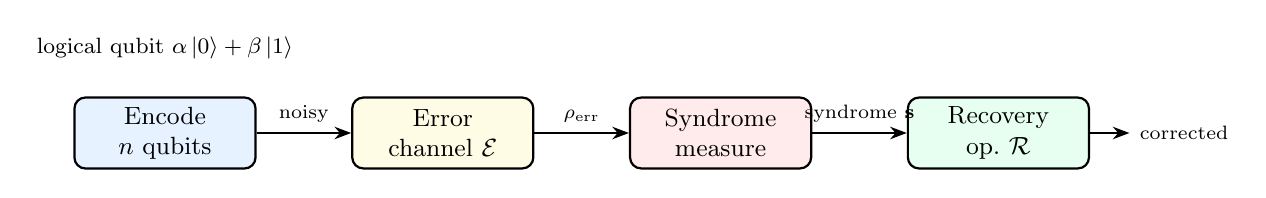
\begin{tikzpicture}[
  box/.style={rectangle, rounded corners=4pt, draw, thick,
              minimum width=2.3cm, minimum height=0.9cm,
              align=center, font=\small},
  arr/.style={-{Stealth[length=6pt]}, thick},
  lbl/.style={font=\scriptsize, align=center}
]
  \node[box, fill=lightblue]  (enc) {Encode \\ $n$ qubits};
  \node[box, fill=lightyellow, right=1.2cm of enc]  (err) {Error \\ channel $\mathcal{E}$};
  \node[box, fill=lightred,   right=1.2cm of err] (syn) {Syndrome \\ measure};
  \node[box, fill=lightgreen, right=1.2cm of syn] (rec) {Recovery \\ op.\ $\mathcal{R}$};

  \draw[arr] (enc) -- (err) node[midway,above,lbl]{noisy};
  \draw[arr] (err) -- (syn) node[midway,above,lbl]{$\rho_{\text{err}}$};
  \draw[arr] (syn) -- (rec) node[midway,above,lbl]{syndrome $\mathbf{s}$};
  \draw[arr] (rec.east) -- ++(0.5,0) node[right,lbl]{corrected};

  \node[above=0.35cm of enc, font=\footnotesize] {logical qubit $\alpha\ket{0}+\beta\ket{1}$};
\end{tikzpicture}
\caption{The three-step QEC pipeline.  The logical qubit is first encoded into
$n$ physical qubits.  After an error channel acts, the syndrome is measured
(without disturbing $\alpha,\beta$), and a recovery operation restores the
original state.}
\label{fig:qec-pipeline}
\end{figure}

\subsection{Historical Context}

Quantum error correction emerged in the mid-1990s in rapid succession:

\begin{itemize}
  \item \textbf{Shor (1995):} First QEC code --- a 9-qubit code correcting
        arbitrary single-qubit errors.
  \item \textbf{Steane (1996):} 7-qubit CSS code derived from classical
        Hamming codes; simpler and more efficient.
  \item \textbf{Knill \& Laflamme (1997):} General algebraic conditions
        (the KL conditions) characterising when a set of errors is
        correctable.
  \item \textbf{Kitaev (1997):} Toric/surface code --- topological QEC with
        local stabilizers, high threshold, and deep connections to topology.
  \item \textbf{Preskill (1997--2012):} Threshold theorem and fault-tolerant
        computing framework.
\end{itemize}

\subsection{Learning Goals for This Chapter}

After reading this chapter, you should be able to:
\begin{itemize}
  \item Calculate the probability that an unprotected quantum computation
        fails due to accumulated errors.
  \item State and prove the no-cloning theorem and explain why it does
        \emph{not} forbid QEC.
  \item Describe the encode--syndrome--recover strategy in plain language.
  \item Explain the three fundamental obstacles preventing direct application
        of classical error correction to qubits.
\end{itemize}

\begin{exercise}
A quantum algorithm requires $n = 500$ two-qubit gates, each with error
probability $p = 0.005$.  What is the probability that no error occurs?
What is the minimum gate fidelity required to ensure the computation
succeeds with probability at least 0.9?
\end{exercise}

\begin{exercise}
Prove that the no-cloning theorem forbids \emph{broadcasting}: there is no
quantum channel $\mathcal{E}$ such that
$\mathcal{E}(\proj{\psi}) = \proj{\psi} \otimes \proj{\psi}$ for all pure
states $\ket{\psi}$.  (\emph{Hint:} use a linearity argument rather than
unitarity.)
\end{exercise}

\begin{exercise}
Explain in your own words why the no-cloning theorem does \emph{not} prevent
quantum error correction.  What feature of QEC allows it to protect
information without copying it?
\end{exercise}

\begin{summarybox}
\textbf{Section 1 key points:}
\begin{itemize}
  \item Qubit errors accumulate rapidly; even 0.1\% gate error makes a
        1000-gate algorithm unreliable without correction.
  \item No-cloning theorem: we cannot copy an unknown quantum state.
  \item QEC works by encoding into entangled states, measuring syndromes
        (error indicators without revealing logical information), and
        applying corrective operations.
\end{itemize}
\end{summarybox}

% ======================================================================
% SECTION 2: QUANTUM ERRORS AND PAULI OPERATORS
% ======================================================================
\newpage
\section{Quantum Errors and the Pauli Framework}
\label{sec:errors}

\begin{intuition}
A single qubit lives on the surface of the ``Bloch sphere'' --- a unit sphere
where the north pole is $\ket{0}$, the south pole is $\ket{1}$, and every
other point is a superposition.  An error is a rotation of this sphere.
There are rotations about three axes: $X$ (flips $\ket{0}\leftrightarrow
\ket{1}$, the ``equatorial flip''), $Z$ (flips the relative phase, a rotation
about the vertical axis), and $Y$ (combines both).  Any rotation can be
decomposed into these three generators --- this is the key insight that makes
discrete error correction possible.
\end{intuition}

\subsection{Single-Qubit Error Types}

Consider a qubit in state $\ket{\psi} = \alpha\ket{0} + \beta\ket{1}$.
Three ``pure'' error types cover all possibilities:

\begin{center}
\renewcommand{\arraystretch}{1.4}
\begin{tabular}{@{} l l l p{5.5cm} @{}}
  \toprule
  \textbf{Error} & \textbf{Op.} & \textbf{Action} & \textbf{Physical meaning}\\
  \midrule
  Bit-flip   & $X$ & $\ket{0}\leftrightarrow\ket{1}$ &
      Like a classical bit-flip; flips amplitude\\
  Phase-flip & $Z$ & $\ket{0}\mapsto\ket{0}$, $\ket{1}\mapsto{-}\ket{1}$ &
      Relative phase flips sign; no classical analogue\\
  Bit+Phase  & $Y{=}iXZ$ & $\ket{0}\mapsto i\ket{1}$, $\ket{1}\mapsto{-}i\ket{0}$ &
      Both effects simultaneously\\
  \bottomrule
\end{tabular}
\end{center}

\subsection{Pauli Matrices}

The four \textbf{Pauli operators} are:
\[
  I = \begin{pmatrix}1&0\\0&1\end{pmatrix},\quad
  X = \begin{pmatrix}0&1\\1&0\end{pmatrix},\quad
  Y = \begin{pmatrix}0&-i\\i&0\end{pmatrix},\quad
  Z = \begin{pmatrix}1&0\\0&-1\end{pmatrix}.
\]
They are Hermitian ($P^\dagger = P$), unitary ($P^\dagger P = I$), and
traceless for $P \in \{X,Y,Z\}$.  Their key algebraic properties are:
\begin{align}
  X^2 = Y^2 = Z^2 &= I, \label{eq:pauli-square}\\
  XY = iZ,\quad YZ = iX,\quad ZX &= iY, \label{eq:pauli-product}\\
  \{X,Z\} = XZ + ZX &= 0 \quad (\text{anticommute}), \label{eq:anticommute}
\end{align}
and similarly for all distinct pairs.  The Paulis \emph{commute} with
themselves and \emph{anticommute} with each other.

\begin{workedexample}[Verifying Pauli algebra]
Let us verify $XZ = -ZX = iY$ directly using matrix multiplication:
\[
  XZ = \begin{pmatrix}0&1\\1&0\end{pmatrix}\begin{pmatrix}1&0\\0&-1\end{pmatrix}
     = \begin{pmatrix}0&-1\\1&0\end{pmatrix},
\]
\[
  ZX = \begin{pmatrix}1&0\\0&-1\end{pmatrix}\begin{pmatrix}0&1\\1&0\end{pmatrix}
     = \begin{pmatrix}0&1\\-1&0\end{pmatrix},
\]
so indeed $XZ = -ZX$.  And:
\[
  iY = i\begin{pmatrix}0&-i\\i&0\end{pmatrix} = \begin{pmatrix}0&1\\-1&0\end{pmatrix}
     = ZX,
\]
confirming $XZ = -ZX = iY$. \hfill$\square$
\end{workedexample}

\subsection{Discretisation of Quantum Errors}
\label{sec:discretisation}

This is one of the most important and surprising facts in quantum error
correction.

\begin{theorem}[Discretisation of Errors]
\label{thm:discretisation}
Any single-qubit error $E$ can be written as a linear combination of Pauli
operators:
\[
  E = c_0 I + c_1 X + c_2 Y + c_3 Z, \qquad c_i \in \mathbb{C}.
\]
Consequently, if a quantum code can correct all single-qubit Pauli errors
$\{I, X, Y, Z\}$, it can correct \textbf{any} single-qubit error.
\end{theorem}

\begin{proof}[Proof sketch]
The four Pauli matrices form a basis for the vector space of $2\times 2$
complex matrices (dimension 4 over $\mathbb{C}$, dimension 4 over $\mathbb{R}$
when restricted to Hermitian matrices).  Any $2\times 2$ matrix $E$ can
therefore be decomposed as stated.  When the syndrome is measured, the
measurement projects the error onto one of its Pauli components (by the
postulates of quantum measurement).  The remaining component is a pure Pauli
error, which the code corrects.
\end{proof}

\begin{intuition}
Think of it like this: your code might only know how to handle three
``standard'' faults (call them X, Y, Z).  When some exotic fault $E$ happens,
\emph{the act of checking which standard fault occurred} forces the actual
error to collapse into one of those standard faults.  After the check, you
have an ordinary fault you already know how to fix.  This is the magic of
quantum measurement used constructively.
\end{intuition}

\begin{workedexample}[Decomposing a rotation error]
A common physical error is an \textbf{over-rotation}: the qubit rotates by
$\theta$ about the $X$-axis instead of not rotating at all.  The error
operator is
\[
  E(\theta) = e^{-i\theta X/2}
            = \cos(\theta/2)\, I - i\sin(\theta/2)\, X.
\]
This is already in Pauli form with $c_0 = \cos(\theta/2)$ and
$c_1 = -i\sin(\theta/2)$.

For a small rotation $\theta = 0.1$ radians:
\[
  c_0 = \cos(0.05) \approx 0.9988, \qquad
  c_1 = -i\sin(0.05) \approx -0.0500\,i.
\]
When the syndrome is measured, the error collapses to $I$ (no error,
probability $|c_0|^2 \approx 0.998$) or $X$ (bit-flip, probability
$|c_1|^2 \approx 0.0025$).  A code that corrects $X$-errors handles
\emph{both outcomes} correctly.
\end{workedexample}

\subsection{Quantum Channels and Kraus Operators}

A more general description of noise uses \textbf{quantum channels}:
\[
  \mathcal{E}(\rho) = \sum_i E_i \rho E_i^\dagger,
  \qquad \sum_i E_i^\dagger E_i = I,
\]
where $\{E_i\}$ are \textbf{Kraus operators}.  Key examples:

\paragraph{Depolarising channel}
With probability $1-p$ nothing happens; otherwise a Pauli error
$X, Y, Z$ each occurs with probability $p/3$:
\[
  \mathcal{E}_{\text{dep}}(\rho)
  = (1-p)\rho + \frac{p}{3}(X\rho X + Y\rho Y + Z\rho Z).
\]

\paragraph{Dephasing (phase-damping) channel}
Only $Z$-errors occur, with probability $p$:
\[
  \mathcal{E}_{\text{deph}}(\rho)
  = (1-p)\rho + p\, Z\rho Z.
\]

\paragraph{Amplitude damping channel}
Models energy relaxation ($T_1$ decay), with Kraus operators:
\[
  K_0 = \begin{pmatrix}1&0\\0&\sqrt{1-\gamma}\end{pmatrix},\quad
  K_1 = \begin{pmatrix}0&\sqrt{\gamma}\\0&0\end{pmatrix},
\]
where $\gamma = 1 - e^{-t/T_1}$ is the decay probability.

\begin{workedexample}[Depolarising channel on $\ket{+}$]
Let $\ket{+} = \tfrac{1}{\sqrt{2}}(\ket{0}+\ket{1})$ so
$\rho = \proj{+} = \tfrac{1}{2}\begin{pmatrix}1&1\\1&1\end{pmatrix}$.

Apply the depolarising channel with $p = 0.12$:
\begin{align*}
  X\rho X &= \frac{1}{2}\begin{pmatrix}1&1\\1&1\end{pmatrix} = \rho
            & (\ket{+}\text{ is a }+1\text{ eigenstate of }X),\\
  Y\rho Y &= \frac{1}{2}\begin{pmatrix}1&-1\\-1&1\end{pmatrix}
            = \proj{-},\\
  Z\rho Z &= \frac{1}{2}\begin{pmatrix}1&-1\\-1&1\end{pmatrix}
            = \proj{-}.
\end{align*}
Therefore:
\[
  \mathcal{E}(\rho)
  = 0.88\,\rho + 0.04\,\rho + 0.04\,\proj{-} + 0.04\,\proj{-}
  = 0.92\,\rho + 0.08\,\proj{-}.
\]
The off-diagonal coherences are reduced: the channel has partially
\emph{dephased} the state in the $\{\ket{+},\ket{-}\}$ basis.
\end{workedexample}

\subsection{Multi-Qubit Pauli Group}

For $n$ qubits, single-qubit Pauli operators are combined by tensor products.
Notation: $X_1 Z_3$ means $X \otimes I \otimes Z$ on qubits 1, 2, 3.

\begin{definition}[$n$-qubit Pauli group]
$\mathcal{P}_n$ consists of all $n$-fold tensor products of
$\{I,X,Y,Z\}$ with overall phases $\{\pm1, \pm i\}$:
\[
  \mathcal{P}_n = \bigl\{ e^{i\phi}
    P_1 \otimes \cdots \otimes P_n
    \;\big|\; P_j \in \{I,X,Y,Z\},\;
    \phi \in \{0, \tfrac{\pi}{2}, \pi, \tfrac{3\pi}{2}\} \bigr\}.
\]
Its size is $|\mathcal{P}_n| = 4^{n+1}$.
\end{definition}

Two $n$-qubit Paulis $A$ and $B$ either \textbf{commute} ($AB = BA$) or
\textbf{anticommute} ($AB = -BA$).  They anticommute if and only if they
anticommute on an \emph{odd} number of qubit positions.

\begin{workedexample}[Commutation in $\mathcal{P}_2$]
Do $A = X_1 Z_2$ and $B = Z_1 X_2$ commute or anticommute?

At position 1: $X$ and $Z$ anticommute $\to$ contributes a sign $-1$.\\
At position 2: $Z$ and $X$ anticommute $\to$ contributes a sign $-1$.\\
Total sign: $(-1)(-1) = +1$.  Therefore $AB = BA$: they \textbf{commute}.

\medskip
Do $C = X_1 I_2$ and $D = Z_1 Z_2$ commute?

At position 1: $X$ and $Z$ anticommute $\to$ sign $-1$.\\
At position 2: $I$ and $Z$ commute $\to$ sign $+1$.\\
Total sign: $(-1)(+1) = -1$.  Therefore $CD = -DC$: they
\textbf{anticommute}.
\end{workedexample}

\subsection{Error Propagation in Circuits}

Errors in gates can \emph{propagate} to other qubits:

\begin{itemize}
  \item An $X$ error on the \emph{control} qubit of a CNOT propagates to
        both the control and target ($X_c \to X_c X_t$).
  \item A $Z$ error on the \emph{target} qubit of a CNOT propagates to
        both ($Z_t \to Z_c Z_t$).
\end{itemize}

\begin{figure}[H]
\centering
\begin{minipage}{0.45\textwidth}
\centering
\begin{quantikz}[column sep=0.5cm]
  \lstick{$\ket{\psi_c}$} & \gate{X_{\text{err}}} & \ctrl{1} & \qw\\
  \lstick{$\ket{\psi_t}$} & \qw & \targ{} & \qw
\end{quantikz}\\[4pt]
{\small $X$ error on control $\to$ $X$ on both}
\end{minipage}
\hfill
\begin{minipage}{0.45\textwidth}
\centering
\begin{quantikz}[column sep=0.5cm]
  \lstick{$\ket{\psi_c}$} & \qw & \ctrl{1} & \qw\\
  \lstick{$\ket{\psi_t}$} & \qw & \targ{} & \gate{Z_{\text{err}}}
\end{quantikz}\\[4pt]
{\small $Z$ error on target $\to$ $Z$ on both}
\end{minipage}
\caption{Error propagation through CNOT: an $X$ error on the control
spreads to the target; a $Z$ error on the target spreads to the control.}
\label{fig:cnot-errors}
\end{figure}

This motivates careful \textbf{fault-tolerant circuit design} covered in
Section~\ref{sec:fault-tolerant}.

\begin{exercise}
Verify equation~\eqref{eq:pauli-product}: compute $YZ$ and $ZX$ using
matrix multiplication and confirm they equal $iX$ and $iY$ respectively.
\end{exercise}

\begin{exercise}
Show that the Pauli matrices $\{I, X, Y, Z\}$ form a basis for the
space of $2\times2$ complex matrices.  (Hint: show they are linearly
independent and use a dimension argument.)
\end{exercise}

\begin{exercise}
For the depolarising channel $\mathcal{E}_{\text{dep}}$ with $p = 0.06$,
compute $\mathcal{E}(\proj{0})$.  What is the probability of a bit-flip
($X$) error? Of a phase-flip ($Z$) error?
\end{exercise}

\begin{exercise}
Determine whether the following pairs of 2-qubit Pauli operators commute
or anticommute: (a) $X_1 X_2$ and $Z_1 Z_2$;
(b) $X_1 Z_2$ and $X_1 X_2$;
(c) $Y_1 Y_2$ and $X_1 Z_2$.
\end{exercise}

\begin{summarybox}
\textbf{Section 2 key points:}
\begin{itemize}
  \item The three Pauli operators $\{X, Y, Z\}$ describe all single-qubit
        errors; $\{I,X,Y,Z\}$ form a basis for $2\times 2$ matrices.
  \item Any physical error can be decomposed in the Pauli basis; syndrome
        measurement collapses it to a single Pauli.
  \item Two $n$-qubit Paulis commute iff they anticommute on an even number
        of positions.
  \item Errors propagate through CNOT gates --- a key concern for
        fault-tolerant design.
\end{itemize}
\end{summarybox}

% ======================================================================
% SECTION 3: REPETITION CODES
% ======================================================================
\newpage
\section{Classical and Quantum Repetition Codes}
\label{sec:repetition}

\begin{intuition}
The simplest way to protect a bit is to say it three times.  If you tell
three people ``the answer is \textbf{0}'' and one of them mishears it as
``the answer is \textbf{1}'', the other two can overrule the mistake.  This is
a repetition code, and it is the starting point for understanding both
classical and quantum error correction.
\end{intuition}

\subsection{Classical 3-Bit Repetition Code}

The classical 3-bit code is:
\[
  0 \longrightarrow 000, \qquad 1 \longrightarrow 111.
\]

\paragraph{Decoding by majority vote.}
If one bit flips, two of the three bits still agree, and majority voting
recovers the original bit.  If two or more bits flip, majority voting fails.
Assuming each bit flips independently with probability $p$:
\[
  P(\text{logical error}) = \binom{3}{2}p^2(1-p) + \binom{3}{3}p^3
                           = 3p^2(1-p) + p^3 = 3p^2 - 2p^3.
\]
For small $p$, $P(\text{logical error}) \approx 3p^2$, which is much smaller
than the uncoded error rate $p$ when $p \ll 1/3$.

\begin{workedexample}[Classical code improvement]
For $p = 0.05$, the uncoded bit error rate is $0.05 = 5\%$.  With the
3-bit repetition code:
\[
  P(\text{logical error}) = 3(0.05)^2 - 2(0.05)^3
  = 3(0.0025) - 2(0.000125)
  \approx 0.00725 \approx 0.73\%.
\]
A 7-fold improvement in error rate!
\end{workedexample}

\paragraph{Syndrome table for the classical code.}
Rather than majority vote, we can identify the error from \emph{parity
checks}:
\[
  s_1 = \text{bit}_1 \oplus \text{bit}_2, \qquad
  s_2 = \text{bit}_2 \oplus \text{bit}_3.
\]
The syndrome $(s_1, s_2)$ tells us exactly which bit (if any) flipped:

\begin{center}
\renewcommand{\arraystretch}{1.3}
\begin{tabular}{@{} c c c c @{}}
  \toprule
  \textbf{Received} & \textbf{Error} & \textbf{$s_1 = b_1\oplus b_2$} &
    \textbf{$s_2 = b_2\oplus b_3$}\\
  \midrule
  000 (or 111) & None  & 0 & 0\\
  100 (or 011) & Flip bit 1 & 1 & 0\\
  010 (or 101) & Flip bit 2 & 1 & 1\\
  001 (or 110) & Flip bit 3 & 0 & 1\\
  \bottomrule
\end{tabular}
\end{center}

\subsection{Quantum 3-Qubit Bit-Flip Code}

We now lift this idea to the quantum world.  The key difference is that we
must protect a \emph{superposition}:

\begin{align}
  \ket{0}_L &= \ket{000}, \label{eq:3qubit-0}\\
  \ket{1}_L &= \ket{111}, \label{eq:3qubit-1}\\
  \ket{\psi_L} &= \alpha\ket{000} + \beta\ket{111}. \label{eq:3qubit-encoded}
\end{align}

This is \emph{not} three copies of $\ket{\psi}$ (which the no-cloning theorem
forbids).  It is an entangled superposition in which $\alpha$ and $\beta$
live in the global correlations, not in any single qubit.

\subsubsection{Encoding Circuit}

Starting from $\ket{\psi}\ket{0}\ket{0} = (\alpha\ket{0}+\beta\ket{1})\ket{0}\ket{0}$,
two CNOT gates produce the encoded state:

\begin{figure}[H]
\centering
\begin{quantikz}[row sep=0.5cm, column sep=0.6cm]
  \lstick{$\ket{\psi}$} & \ctrl{1} & \ctrl{2} & \qw & \rstick[3]{$\alpha\ket{000}+\beta\ket{111}$}\\
  \lstick{$\ket{0}$}    & \targ{}  & \qw      & \qw\\
  \lstick{$\ket{0}$}    & \qw      & \targ{}  & \qw
\end{quantikz}
\caption{Encoding circuit for the 3-qubit bit-flip code.}
\label{fig:3qubit-encoding}
\end{figure}

\textbf{Trace through:}
\begin{align*}
  (\alpha\ket{0}+\beta\ket{1})\ket{00}
  &\xrightarrow{\text{CNOT}_{1,2}}
    \alpha\ket{000} + \beta\ket{110}\\
  &\xrightarrow{\text{CNOT}_{1,3}}
    \alpha\ket{000} + \beta\ket{111}. \checkmark
\end{align*}

\subsubsection{Quantum Syndrome Measurement}

We measure the \textbf{stabilizers} $g_1 = Z_1 Z_2$ and $g_2 = Z_2 Z_3$
using ancilla qubits.  These operators measure the \emph{parity} of pairs of
data qubits without touching $\alpha$ or $\beta$.

\begin{figure}[H]
\centering
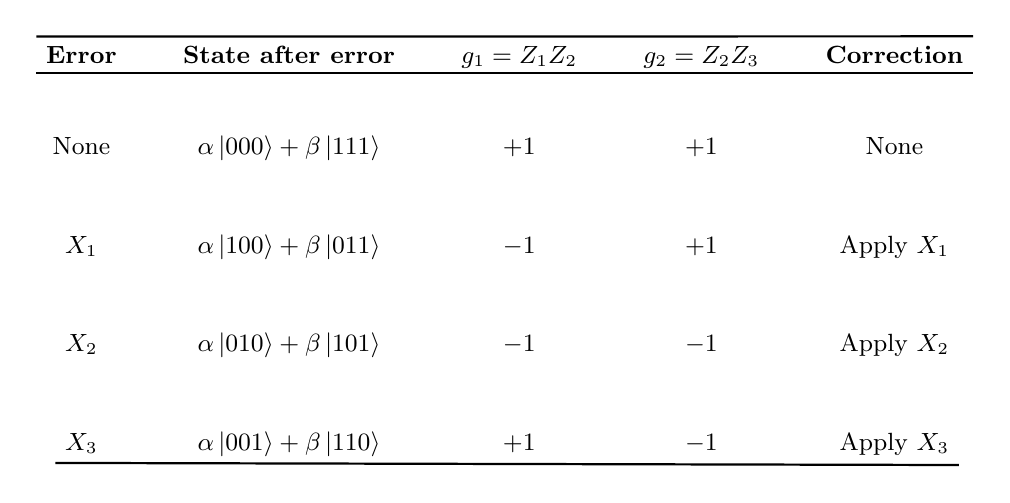
\begin{tikzpicture}[
  box/.style={rectangle, draw, thick, minimum width=1.4cm,
              minimum height=0.6cm, align=center, font=\small},
  every node/.style={font=\small}
]
  \matrix (m) [matrix of nodes, row sep=0.7cm, column sep=0.5cm,
               nodes={align=center}] {
    \textbf{Error} & \textbf{State after error} &
    \textbf{$g_1=Z_1Z_2$} & \textbf{$g_2=Z_2Z_3$} &
    \textbf{Correction}\\[-2pt]
    None & $\alpha\ket{000}+\beta\ket{111}$ & $+1$ & $+1$ & None\\
    $X_1$ & $\alpha\ket{100}+\beta\ket{011}$ & $-1$ & $+1$ & Apply $X_1$\\
    $X_2$ & $\alpha\ket{010}+\beta\ket{101}$ & $-1$ & $-1$ & Apply $X_2$\\
    $X_3$ & $\alpha\ket{001}+\beta\ket{110}$ & $+1$ & $-1$ & Apply $X_3$\\
  };
  \draw[thick] (m-1-1.south west) -- (m-1-5.south east);
  \draw[thick] (m-1-1.north west) -- (m-1-5.north east);
  \draw[thick] (m-5-1.south west) -- (m-5-5.south east);
\end{tikzpicture}
\caption{Syndrome table for the 3-qubit bit-flip code.  The syndrome
$(g_1, g_2)$ uniquely identifies single-qubit bit-flip errors.  Crucially,
$\alpha$ and $\beta$ never appear in the syndrome.}
\label{tab:3qubit-syndrome}
\end{figure}

\begin{workedexample}[Full syndrome computation for $X_2$]
Suppose qubit 2 suffers a bit-flip.  After encoding, the state is
$\alpha\ket{000} + \beta\ket{111}$.  The error $X_2$ (acting on qubit 2) gives:
\[
  \text{State after error: }
  X_2\bigl(\alpha\ket{000}+\beta\ket{111}\bigr)
  = \alpha\ket{010} + \beta\ket{101}.
\]

\textbf{Measuring $g_1 = Z_1 Z_2$:}
\begin{align*}
  Z_1 Z_2 \ket{010} &= Z\ket{0} \otimes Z\ket{1} \otimes I\ket{0}
                    = (+1)(-1)\ket{010} = -\ket{010},\\
  Z_1 Z_2 \ket{101} &= Z\ket{1} \otimes Z\ket{0} \otimes I\ket{1}
                    = (-1)(+1)\ket{101} = -\ket{101}.
\end{align*}
Both terms give eigenvalue $-1$, so the measurement outcome is $g_1 = -1$.

\textbf{Measuring $g_2 = Z_2 Z_3$:}
\begin{align*}
  Z_2 Z_3 \ket{010} &= Z\ket{1} \otimes Z\ket{0} = (-1)(+1) = -1,\\
  Z_2 Z_3 \ket{101} &= Z\ket{0} \otimes Z\ket{1} = (+1)(-1) = -1.
\end{align*}
The measurement outcome is $g_2 = -1$.

\textbf{Syndrome: $(g_1, g_2) = (-1, -1)$.}  From the table, this corresponds
to an $X_2$ error.  We apply $X_2$ to correct:
\[
  X_2\bigl(\alpha\ket{010}+\beta\ket{101}\bigr)
  = \alpha\ket{000}+\beta\ket{111}. \checkmark
\]
The encoded state is perfectly restored.  Note that $\alpha$ and $\beta$
were never measured and are unaffected.
\end{workedexample}

\subsubsection{Full Syndrome Circuit}

\begin{figure}[H]
\centering
\begin{quantikz}[row sep=0.5cm, column sep=0.6cm]
  \lstick[3]{$\alpha\ket{000}+\beta\ket{111}$}
  & \qw & \ctrl{3} & \qw      & \qw      & \qw\\
  & \qw & \qw      & \ctrl{2} & \ctrl{3} & \qw\\
  & \qw & \qw      & \qw      & \qw      & \ctrl{2}\\
  \lstick{$\ket{0}$} & \qw & \targ{}  & \targ{}  & \qw      & \qw
    & \meter{$s_1$}\\
  \lstick{$\ket{0}$} & \qw & \qw      & \qw      & \targ{}  & \targ{}
    & \meter{$s_2$}
\end{quantikz}
\caption{Syndrome measurement circuit for the 3-qubit bit-flip code.
Ancilla qubits measure $Z_1Z_2$ (giving $s_1$) and $Z_2Z_3$ (giving $s_2$)
without disturbing $\alpha\ket{000}+\beta\ket{111}$.}
\label{fig:3qubit-syndrome-circuit}
\end{figure}

\subsection{Limitations: Phase Errors Are Not Corrected}

The 3-qubit bit-flip code protects against $X$ errors but is \emph{blind} to
$Z$ errors.

\begin{workedexample}[Phase flip on qubit 1 is undetected]
Suppose a phase-flip $Z_1$ occurs on the encoded state:
\[
  Z_1\bigl(\alpha\ket{000}+\beta\ket{111}\bigr)
  = \alpha\ket{000} - \beta\ket{111}.
\]
Check the syndrome:
\begin{align*}
  Z_1 Z_2 (\alpha\ket{000}-\beta\ket{111})
  &= \alpha(+1)(+1)\ket{000} - \beta(-1)(-1)\ket{111}\\
  &= \alpha\ket{000}-\beta\ket{111},\quad g_1 = +1,\\
  Z_2 Z_3 (\alpha\ket{000}-\beta\ket{111})
  &= +\alpha\ket{000} - \beta\ket{111},\quad g_2 = +1.
\end{align*}
Syndrome $(+1,+1)$ says ``no error'' --- but the logical state has been
changed from $\alpha\ket{0}_L+\beta\ket{1}_L$ to
$\alpha\ket{0}_L - \beta\ket{1}_L$.  The error is \emph{undetected}.
\end{workedexample}

\subsection{Quantum Phase-Flip Code}

To correct phase errors, we move to the \emph{Hadamard basis}
$\{\ket{+}, \ket{-}\}$:
\[
  \ket{+} = \frac{\ket{0}+\ket{1}}{\sqrt{2}}, \qquad
  \ket{-} = \frac{\ket{0}-\ket{1}}{\sqrt{2}}.
\]
In this basis, $Z$ errors become $X$ errors: $Z\ket{+} = \ket{-}$ and
$Z\ket{-} = \ket{+}$.

Encode the logical qubit as:
\[
  \ket{0}_L = \ket{+++}, \qquad \ket{1}_L = \ket{---},
\]
so $\ket{\psi}_L = \alpha\ket{+++}+\beta\ket{---}$.

\begin{figure}[H]
\centering
\begin{quantikz}[row sep=0.5cm, column sep=0.6cm]
  \lstick{$\ket{\psi}$} & \ctrl{1} & \ctrl{2} & \gate{H} & \qw\\
  \lstick{$\ket{0}$}    & \targ{}  & \qw      & \gate{H} & \qw\\
  \lstick{$\ket{0}$}    & \qw      & \targ{}  & \gate{H} & \qw
\end{quantikz}
\caption{Phase-flip code encoding: first encode with CNOTs (as in the bit-flip
code), then apply Hadamard to each qubit.}
\label{fig:phase-flip-encoding}
\end{figure}

The stabilizers are now $X_1 X_2$ and $X_2 X_3$ (parity in the Hadamard
basis), detecting $Z$ errors.  The decoding applies $H^{\otimes 3}$ to
convert back, then corrects as before.

\begin{caution}
The phase-flip code corrects $Z$ errors only; the bit-flip code corrects
$X$ errors only.  Neither code corrects both types simultaneously.  For
complete single-qubit error correction, we need a code that handles both ---
this is the \textbf{Shor 9-qubit code} (Section~\ref{sec:shor}).
\end{caution}

\subsection{Why This Works Despite No-Cloning}

A common confusion: if we cannot clone $\ket{\psi}$, how can we store it in
three qubits?  The key is that the encoded state
$\alpha\ket{000}+\beta\ket{111}$ is \emph{not} three copies of $\ket{\psi}$.

\begin{itemize}
  \item Tracing out any one qubit of $\alpha\ket{000}+\beta\ket{111}$ gives
        a \emph{mixed} state (not $\ket{\psi}$).
  \item The information about $\alpha$ and $\beta$ is in the
        \emph{correlations} between the three qubits, not in any single qubit.
  \item Syndrome measurement reveals only the \emph{parity} of pairs, not
        $\alpha$ or $\beta$ individually.
\end{itemize}

\begin{exercise}
Verify that the syndrome $(g_1, g_2) = (+1, -1)$ correctly identifies an
$X_3$ error by carrying out the eigenvalue calculation explicitly.
\end{exercise}

\begin{exercise}
Show that the 3-qubit bit-flip code has \emph{two} possible corrective
operations for each non-trivial syndrome --- for instance, when $(g_1,g_2)
= (-1, +1)$ you might apply $X_1$.  Why does it not matter whether we
apply $X_1$ or instead apply $X_2 X_3$ (which has the same syndrome)?
(\emph{Hint:} what is the product $X_1 \cdot X_2 X_3$ on the encoded
subspace?)
\end{exercise}

\begin{exercise}
Derive the encoding circuit for the quantum phase-flip code by:
(a) showing that $H\ket{0} = \ket{+}$ and $H\ket{1} = \ket{-}$;
(b) tracing $\ket{\psi}\ket{0}\ket{0}$ through the CNOT$+$Hadamard circuit
    to confirm $\ket{0}_L = \ket{+++}$ and $\ket{1}_L = \ket{---}$.
\end{exercise}

\begin{exercise}
Why does the 3-qubit bit-flip code fail to correct a $Y$ error on qubit 2?
Find the syndrome and show that applying the ``correction'' actually
introduces an additional error.
\end{exercise}

\begin{summarybox}
\textbf{Section 3 key points:}
\begin{itemize}
  \item The quantum 3-qubit bit-flip code encodes
        $\alpha\ket{0}+\beta\ket{1}$ as $\alpha\ket{000}+\beta\ket{111}$.
        This is \emph{not} cloning; $\alpha, \beta$ live in correlations.
  \item Syndrome measurement identifies which qubit was flipped without
        disturbing the logical information.
  \item This code protects against $X$ errors \emph{only}; it is blind to
        $Z$ (phase) errors.
  \item The phase-flip code encodes in the Hadamard basis, protecting against
        $Z$ errors only.
  \item A code that corrects both $X$ and $Z$ errors requires a new idea:
        the Shor code.
\end{itemize}
\end{summarybox}

% ======================================================================
% SECTION 4: SHOR 9-QUBIT CODE
% ======================================================================
\newpage
\section{The Shor 9-Qubit Code}
\label{sec:shor}

\begin{intuition}
The 3-qubit bit-flip code fixes $X$ errors; the 3-qubit phase-flip code fixes
$Z$ errors.  Shor's idea was beautifully simple: \emph{concatenate} the two.
First encode the logical qubit into three qubits using the phase-flip code.
Then encode each of those three qubits into three more qubits using the
bit-flip code.  The result is a 9-qubit code that corrects any single-qubit
error.
\end{intuition}

\subsection{Encoding}

The logical codewords are:
\begin{align}
  \ket{0}_L &= \frac{1}{2\sqrt{2}}
    \bigl(\ket{000}+\ket{111}\bigr)^{\otimes 3}, \label{eq:shor-0}\\
  \ket{1}_L &= \frac{1}{2\sqrt{2}}
    \bigl(\ket{000}-\ket{111}\bigr)^{\otimes 3}. \label{eq:shor-1}
\end{align}
Written out:
\begin{align*}
  \ket{0}_L &= \frac{1}{2\sqrt{2}}
    \bigl(\ket{000}+\ket{111}\bigr)
    \bigl(\ket{000}+\ket{111}\bigr)
    \bigl(\ket{000}+\ket{111}\bigr),\\
  \ket{1}_L &= \frac{1}{2\sqrt{2}}
    \bigl(\ket{000}-\ket{111}\bigr)
    \bigl(\ket{000}-\ket{111}\bigr)
    \bigl(\ket{000}-\ket{111}\bigr).
\end{align*}

\subsubsection{Structure of the Encoding}

Figure~\ref{fig:shor-structure} shows the nested structure.

\begin{figure}[H]
\centering
\begin{tikzpicture}[
  outer/.style={draw=blue!70!black, thick, rounded corners=8pt,
                fill=blue!8, inner sep=8pt},
  inner/.style={draw=green!50!black, thick, rounded corners=4pt,
                fill=green!8, inner sep=5pt},
  qbox/.style={draw=orange!70!black, fill=orange!10, rounded corners=2pt,
               minimum width=0.6cm, minimum height=0.6cm, font=\scriptsize},
  label/.style={font=\small}
]
  % Outer phase-flip structure
  \node[outer, label=above:{Phase-flip code block (3 blocks)}] (outer) {%
    \begin{tikzpicture}
      % Block 1
      \node[inner, label=above:{\scriptsize Block 1}] (b1) {%
        \begin{tikzpicture}
          \node[qbox] (q1) {$q_1$};
          \node[qbox, right=0.1cm of q1] (q2) {$q_2$};
          \node[qbox, right=0.1cm of q2] (q3) {$q_3$};
        \end{tikzpicture}
      };
      % Block 2
      \node[inner, right=0.5cm of b1, label=above:{\scriptsize Block 2}] (b2) {%
        \begin{tikzpicture}
          \node[qbox] (q4) {$q_4$};
          \node[qbox, right=0.1cm of q4] (q5) {$q_5$};
          \node[qbox, right=0.1cm of q5] (q6) {$q_6$};
        \end{tikzpicture}
      };
      % Block 3
      \node[inner, right=0.5cm of b2, label=above:{\scriptsize Block 3}] (b3) {%
        \begin{tikzpicture}
          \node[qbox] (q7) {$q_7$};
          \node[qbox, right=0.1cm of q7] (q8) {$q_8$};
          \node[qbox, right=0.1cm of q8] (q9) {$q_9$};
        \end{tikzpicture}
      };
    \end{tikzpicture}
  };

  % Annotations
  \draw[<->, thick, orange!70!black] ($ (outer.south west) + (0.35,-0.3) $)
    -- node[below, font=\small] {bit-flip code within each block}
    ($ (outer.south east) + (-0.35,-0.3) $);
  \draw[<->, thick, blue!70!black] ($ (outer.west) + (-0.1,0) $)
    -- node[left, font=\small, align=right] {phase-flip\\code\\across\\blocks}
    ($ (outer.west) + (-0.1,-2.0) $);
\end{tikzpicture}
\caption{The nested structure of the Shor 9-qubit code.  Three groups of
three qubits each form a bit-flip code.  Across the three groups, the overall
structure forms a phase-flip code.}
\label{fig:shor-structure}
\end{figure}

\subsubsection{Encoding Circuit}

\begin{figure}[H]
\centering
\scalebox{0.85}{%
\begin{quantikz}[row sep=0.35cm, column sep=0.5cm]
  \lstick{$\ket{\psi}$}
    & \ctrl{3} & \ctrl{6}
    & \gate{H} & \ctrl{1} & \ctrl{2} & \qw\\
  \lstick{$\ket{0}$} & \qw & \qw & \qw & \qw & \qw & \qw\\
  \lstick{$\ket{0}$} & \qw & \qw & \qw & \qw & \qw & \qw\\
  \lstick{$\ket{0}$} & \targ{} & \qw
    & \gate{H} & \ctrl{1} & \ctrl{2} & \qw\\
  \lstick{$\ket{0}$} & \qw & \qw & \qw & \qw & \qw & \qw\\
  \lstick{$\ket{0}$} & \qw & \qw & \qw & \qw & \qw & \qw\\
  \lstick{$\ket{0}$} & \qw & \targ{}
    & \gate{H} & \ctrl{1} & \ctrl{2} & \qw\\
  \lstick{$\ket{0}$} & \qw & \qw & \qw & \qw & \qw & \qw\\
  \lstick{$\ket{0}$} & \qw & \qw & \qw & \qw & \qw & \qw
\end{quantikz}}
\caption{Shor code encoding circuit (simplified).  First two CNOTs copy the
logical qubit to qubits 4 and 7 (phase-flip structure).  Then Hadamards
create superpositions.  Finally CNOTs within each block of three create the
bit-flip structure.  Rows 2--3, 5--6, 8--9 receive the CNOT targets from
their respective block leaders.}
\label{fig:shor-encoding}
\end{figure}

\subsection{Stabilizer Generators}
\label{sec:shor-stabilizers}

The Shor code is a stabilizer code (see Section~\ref{sec:stabilizer}).
Its 8 independent generators are:

\subsubsection{Bit-flip stabilizers (within each 3-qubit block)}

\[
  g_1 = Z_1 Z_2,\quad g_2 = Z_2 Z_3,\quad
  g_3 = Z_4 Z_5,\quad g_4 = Z_5 Z_6,\quad
  g_5 = Z_7 Z_8,\quad g_6 = Z_8 Z_9.
\]

Each $Z_i Z_j$ detects an $X$ error on qubit $i$ or $j$ within its block
(a ``parity check'' in the computational basis).

\subsubsection{Phase-flip stabilizers (across blocks)}

\[
  g_7 = X_1 X_2 X_3 X_4 X_5 X_6,\qquad
  g_8 = X_1 X_2 X_3 X_7 X_8 X_9.
\]

These 6-qubit operators detect relative phase errors \emph{between} the
three blocks.

\begin{keypoint}
Eight generators for 9 qubits leave $2^{9-8} = 2$ code states --- encoding
exactly 1 logical qubit.  All 8 generators commute pairwise (necessary for
a valid stabilizer code).
\end{keypoint}

\subsection{Error Correction Capability}

\begin{workedexample}[Correcting a bit-flip on qubit 5]
Suppose $X_5$ occurs.  State after error:
$X_5\ket{\psi_L}$ (some modified encoded state).

\textbf{Bit-flip stabilizers for block 2:}
\begin{align*}
  g_3 = Z_4 Z_5: &\quad Z_4 \text{ commutes with } X_5,\;
    Z_5 \text{ anticommutes with } X_5 \Rightarrow g_3 = -1.\\
  g_4 = Z_5 Z_6: &\quad Z_5 \text{ anticommutes with } X_5,\;
    Z_6 \text{ commutes} \Rightarrow g_4 = -1.
\end{align*}
All other generators commute with $X_5$ (they act on different qubits or
commute position-by-position), giving $+1$.

\textbf{Syndrome:} $g_3 = -1$, $g_4 = -1$, all others $= +1$.  This
uniquely identifies qubit 5 in block 2.  Apply $X_5$ to correct.
\end{workedexample}

\begin{workedexample}[Correcting a phase-flip on qubit 2]
Suppose $Z_2$ occurs.  We check the phase stabilizers:

$Z_2$ anticommutes with $X_2$ (a factor in both $g_7$ and $g_8$), so
both $g_7$ and $g_8$ flip sign: $g_7 = -1$, $g_8 = -1$.

The bit-flip stabilizers $g_1 = Z_1 Z_2$ and $g_2 = Z_2 Z_3$: does $Z_2$
commute with $Z_1 Z_2$?  Yes: $Z_2 \cdot Z_1 Z_2 = Z_1 Z_2^2 = Z_1$, but
since we are checking whether $Z_2$ commutes with $g_1$ as an \emph{operator},
note that $Z_2$ and $Z_j$ always commute (both are $Z$-type).  So the
bit-flip stabilizers all give $+1$.

\textbf{Syndrome:} $g_7 = g_8 = -1$, others $+1$.  This indicates a
phase flip in block 1 (blocks 1 and 2 relative to block 3).  We apply a
correction operator to fix the phase.
\end{workedexample}

\subsection{Correcting Arbitrary Single-Qubit Errors}

Any single-qubit error $E = c_0 I + c_1 X + c_2 Y + c_3 Z$ on any one of
the 9 qubits can be corrected:

\begin{enumerate}
  \item $I$: trivial (no error).
  \item $X$ on qubit $j$: identified by bit-flip stabilizers of the block
        containing $j$.
  \item $Z$ on qubit $j$: identified by phase stabilizers $g_7, g_8$
        (relative signs between blocks tell us which block, bit-flip
        stabilizers within the block locate the qubit).
  \item $Y = iXZ$: produces both $X$- and $Z$-type syndrome outcomes
        simultaneously; both are corrected.
\end{enumerate}

\subsection{Logical Operators}

The logical operators acting on the encoded qubit are:
\[
  \bar{X} = X_1 X_2 X_3 X_4 X_5 X_6 X_7 X_8 X_9
          = X^{\otimes 9},
\]
\[
  \bar{Z} = Z_1 Z_2 Z_3.
\]
(Any $Z_j Z_k Z_l$ with one qubit from each block also works for $\bar{Z}$.)

\begin{exercise}
Verify that $g_7$ and $g_8$ commute.  (\emph{Hint:} they share 3 common
$X$-positions; count how many positions they anticommute.)
\end{exercise}

\begin{exercise}
Show that $\bar{Z} = Z_1 Z_2 Z_3$ commutes with all 8 stabilizer generators
but is not itself in the stabilizer group.
\end{exercise}

\begin{exercise}
Why does the Shor code use 9 qubits and not 7?  Research (or argue from
first principles) why the code distance must be at least 3 to correct any
single-qubit error.
\end{exercise}

\begin{summarybox}
\textbf{Section 4 key points:}
\begin{itemize}
  \item The Shor code combines a phase-flip code (3 blocks) with a bit-flip
        code (within each block) to correct any single-qubit error.
  \item It uses 9 physical qubits to encode 1 logical qubit.
  \item 8 stabilizer generators (6 $ZZ$-type, 2 $XXXXXX$-type) produce 8
        syndrome bits, uniquely identifying all single-qubit Pauli errors.
  \item Any continuous single-qubit error is corrected via discretisation.
\end{itemize}
\end{summarybox}

% ======================================================================
% SECTION 5: STEANE 7-QUBIT CODE
% ======================================================================
\newpage
\section{The Steane $\code{7,1,3}$ Code}
\label{sec:steane}

\begin{intuition}
The Shor code is a beautiful proof of concept, but it is rather wasteful:
9 physical qubits for 1 logical qubit.  The Steane code achieves the same
goal with only 7 qubits, using a deep connection between quantum codes and
classical coding theory.  The idea is to take a classical error-correcting
code (the Hamming code) and ``lift'' it to the quantum world using a
construction called CSS (Calderbank--Shor--Steane).
\end{intuition}

\subsection{The Classical Hamming $[7,4,3]$ Code}

The classical \textbf{Hamming code} $[7,4,3]$ encodes 4 data bits into 7
bits, correcting 1-bit errors.  Its $3\times 7$ parity-check matrix is:

\[
  H = \begin{pmatrix}
    1 & 0 & 0 & 1 & 0 & 1 & 1 \\
    0 & 1 & 0 & 1 & 1 & 0 & 1 \\
    0 & 0 & 1 & 0 & 1 & 1 & 1
  \end{pmatrix}.
\]

\begin{itemize}
  \item A codeword $\mathbf{c}$ satisfies $H\mathbf{c}^T = \mathbf{0}$
        (all parities are even).
  \item The syndrome $H\mathbf{e}^T$ of an error $\mathbf{e}$ is the
        binary representation of the position of the flipped bit.
  \item Distance $d = 3$: any two codewords differ in at least 3 bits,
        so 1-bit errors can always be corrected.
\end{itemize}

\begin{workedexample}[Hamming code syndrome]
Suppose we transmit the codeword $\mathbf{c} = (1,0,1,0,1,0,0)$ but
receive $\mathbf{r} = (1,0,\mathbf{0},0,1,0,0)$ (bit 3 flipped).
Compute the syndrome:
\[
  H\mathbf{r}^T
  = \begin{pmatrix}1\\0\\0\end{pmatrix}\cdot 1
  + \begin{pmatrix}0\\0\\1\end{pmatrix}\cdot 0 \cdots
  = \begin{pmatrix}0\\0\\1\end{pmatrix},
\]
which in binary is $(001)_2 = 3$.  So bit position 3 was flipped.
Correcting it recovers $\mathbf{c}$.
\end{workedexample}

\subsection{The CSS Construction}

\begin{definition}[CSS code]
Given classical linear codes $C_1 \supseteq C_2$ with parity-check matrices
$H_1$ and $H_2$, the \textbf{CSS code} $\text{CSS}(C_1, C_2)$ is a quantum
code with stabilizers:
\begin{itemize}
  \item $X$-type: one $X^{\otimes \text{row}}$ generator per row of $H_2$,
  \item $Z$-type: one $Z^{\otimes \text{row}}$ generator per row of $H_1$.
\end{itemize}
The construction is valid (all generators commute) if and only if
$H_1 H_2^T = 0$ over $\mathbb{F}_2$.
\end{definition}

\subsection{Steane Code Construction}

The Steane code uses the Hamming $[7,4,3]$ code with $H_1 = H_2 = H$.
Crucially, $H H^T = 0 \pmod{2}$ (verify this!), so the CSS condition is
satisfied.

\subsubsection{Stabilizer Generators}

Each row of $H$ defines both an $X$-type and a $Z$-type stabilizer by
placing $X$ (or $Z$) on qubit $j$ wherever the row has a 1:

\textbf{Row 1:} $(1,0,0,1,0,1,1)$ acts on qubits 1, 4, 6, 7.\\
\textbf{Row 2:} $(0,1,0,1,1,0,1)$ acts on qubits 2, 4, 5, 7.\\
\textbf{Row 3:} $(0,0,1,0,1,1,1)$ acts on qubits 3, 5, 6, 7.

This gives 6 generators in total:

\[
\begin{array}{rl}
  g_1 &= X_1 X_4 X_6 X_7,\\
  g_2 &= X_2 X_4 X_5 X_7,\\
  g_3 &= X_3 X_5 X_6 X_7,
\end{array}
\qquad
\begin{array}{rl}
  g_4 &= Z_1 Z_4 Z_6 Z_7,\\
  g_5 &= Z_2 Z_4 Z_5 Z_7,\\
  g_6 &= Z_3 Z_5 Z_6 Z_7.
\end{array}
\]

\begin{keypoint}
For any CSS code, $X$-type and $Z$-type generators always commute: an
$X$-type generator and a $Z$-type generator acting on the same qubits
must anticommute on an \emph{even} number of positions, because
$H_1 H_2^T = 0$ means their supports overlap in an even number of
positions.
\end{keypoint}

\subsubsection{Code Parameters}

\begin{center}
\renewcommand{\arraystretch}{1.3}
\begin{tabular}{@{} l c l @{}}
  \toprule
  \textbf{Parameter} & \textbf{Value} & \textbf{Meaning}\\
  \midrule
  $n$ & 7 & physical qubits\\
  $k$ & 1 & logical qubits encoded ($= n - \text{number of generators} = 7-6$)\\
  $d$ & 3 & code distance (corrects $\lfloor(d-1)/2\rfloor = 1$ error)\\
  \bottomrule
\end{tabular}
\end{center}

\subsection{Logical Operators}

\[
  \bar{X} = X_1 X_2 X_3 X_4 X_5 X_6 X_7 = X^{\otimes 7},
\]
\[
  \bar{Z} = Z_1 Z_2 Z_3 Z_4 Z_5 Z_6 Z_7 = Z^{\otimes 7}.
\]
These are the minimum-weight logical operators (weight 7, which equals the
distance $d$ --- as expected).

\subsection{Error Correction Procedure}

\begin{workedexample}[Detecting a $Z$-error on qubit 3]
Suppose $Z_3$ occurs.  We check the $X$-type stabilizers:
\begin{align*}
  g_1 = X_1 X_4 X_6 X_7: & \quad Z_3 \text{ does not act on qubits 1,4,6,7}
    \Rightarrow \text{commutes} \Rightarrow +1.\\
  g_2 = X_2 X_4 X_5 X_7: & \quad Z_3 \text{ not on these qubits}
    \Rightarrow +1.\\
  g_3 = X_3 X_5 X_6 X_7: & \quad Z_3 \text{ acts on qubit 3, }
    Z \text{ anticommutes with } X \Rightarrow -1.
\end{align*}

The $Z$-type stabilizers all commute with $Z_3$ (same Pauli type), giving
$+1$.

\textbf{$X$-syndrome:} $(g_1, g_2, g_3) = (+1, +1, -1)$.  In binary $(0,0,1)$,
which encodes the position $001_2 = 1$... but we need to match the Hamming
matrix convention.  Row 3 of $H$ is $(0,0,1,0,1,1,1)$, which has a 1 in
position 3, confirming the error is on qubit 3.  Apply $Z_3$ to correct.
\end{workedexample}

\subsection{Transversal Gates}

A major advantage of the Steane code is its support for \textbf{transversal}
gates --- operations that apply identically to each physical qubit:

\begin{center}
\renewcommand{\arraystretch}{1.4}
\begin{tabular}{@{} l c l @{}}
  \toprule
  \textbf{Logical gate} & \textbf{Physical implementation} & \textbf{Why it works}\\
  \midrule
  $\bar{H}$ (Hadamard) & $H^{\otimes 7}$ & Steane code is self-dual ($H_X = H_Z$)\\
  $\bar{S}$ (Phase gate) & $S^{\otimes 7}$ & CSS structure preserved\\
  $\overline{\text{CNOT}}$ & $\text{CNOT}^{\otimes 7}$ & Bitwise CNOT between two code blocks\\
  \bottomrule
\end{tabular}
\end{center}

These three gates generate the \textbf{Clifford group}, which is a rich but
not universal gate set.

\begin{caution}
The $T$ gate ($T = \text{diag}(1, e^{i\pi/4})$) is \emph{not} transversal in
the Steane code because $T^{\otimes 7}$ does not preserve the code space.
Implementing a fault-tolerant $T$ gate requires \textbf{magic state
distillation} (Section~\ref{sec:magic}).  This is one of the main overhead
costs of fault-tolerant quantum computation.
\end{caution}

\begin{exercise}
Verify that $H H^T = 0 \pmod{2}$ for the Hamming matrix $H$ given above.
This is the CSS construction validity condition.
\end{exercise}

\begin{exercise}
Compute the $Z$-syndrome (outcomes of $g_4, g_5, g_6$) when an $X$-error
occurs on qubit 5.  Confirm it correctly identifies qubit 5.
\end{exercise}

\begin{exercise}
Explain why the Steane code needs only 7 qubits while the Shor code needs 9
to correct the same set of errors.  What property of the Hamming code makes
this possible?
\end{exercise}

\begin{summarybox}
\textbf{Section 5 key points:}
\begin{itemize}
  \item The Steane code is a $\code{7,1,3}$ CSS code derived from the
        classical Hamming $[7,4,3]$ code.
  \item Its 6 stabilizer generators (3 $X$-type, 3 $Z$-type) come directly
        from the rows of the Hamming parity-check matrix.
  \item $X$-type and $Z$-type generators always commute in a CSS code.
  \item The code admits transversal Hadamard, Phase, and CNOT --- the full
        Clifford group --- but not the $T$ gate.
\end{itemize}
\end{summarybox}

% ======================================================================
% SECTION 6: STABILIZER FORMALISM
% ======================================================================
\newpage
\section{The Stabilizer Formalism}
\label{sec:stabilizer}

\begin{intuition}
The 3-qubit, Shor, and Steane codes all share a common structure: there is a
set of multi-qubit Pauli operators (the \emph{stabilizers}) that all
codewords satisfy simultaneously.  Errors shift codewords out of this
``eigenspace'', and measuring the stabilizers --- without touching the
logical information --- tells you what went wrong.  The stabilizer formalism
is the mathematical framework that unifies all these examples and provides a
systematic way to construct and analyse quantum codes.
\end{intuition}

\subsection{The Pauli Group (Reminder)}

The $n$-qubit Pauli group $\mathcal{P}_n$ was defined in
Section~\ref{sec:errors}.  Its key properties:
\begin{itemize}
  \item Every element squares to $\pm I$.
  \item Any two elements either commute or anticommute.
  \item Elements can be described efficiently: an $n$-qubit Pauli is
        specified by two $n$-bit strings $(a, b)$ where $a_j = 1$ means
        $X_j$ appears and $b_j = 1$ means $Z_j$ appears (with $Y_j = iX_jZ_j$
        when both are 1), plus a phase.
\end{itemize}

\subsection{Definition of a Stabilizer Code}

\begin{definition}[Stabilizer group and code space]
An abelian subgroup $S \leq \mathcal{P}_n$ not containing $-I$ is called
a \textbf{stabilizer group}.  The associated \textbf{code space} is the
simultaneous $+1$ eigenspace:
\[
  \mathcal{C}(S)
  = \bigl\{\, \ket{\psi} \in (\mathbb{C}^2)^{\otimes n}
    \;\big|\; s\ket{\psi} = +\ket{\psi},\;\forall s \in S \bigr\}.
\]
\end{definition}

If $S$ is generated by $n-k$ independent generators
$\{g_1, \dots, g_{n-k}\}$, then $\dim \mathcal{C}(S) = 2^k$, encoding
$k$ logical qubits into $n$ physical qubits.

\begin{workedexample}[Verifying the 3-qubit code space]
The 3-qubit bit-flip code has stabilizer $S = \langle Z_1Z_2, Z_2Z_3 \rangle$.
We check that $\ket{000}$ and $\ket{111}$ are in the code space:
\begin{align*}
  Z_1 Z_2 \ket{000} &= (+1)(+1)\ket{000} = +\ket{000}, \checkmark\\
  Z_2 Z_3 \ket{000} &= (+1)(+1)\ket{000} = +\ket{000}, \checkmark\\
  Z_1 Z_2 \ket{111} &= (-1)(-1)\ket{111} = +\ket{111}, \checkmark\\
  Z_2 Z_3 \ket{111} &= (-1)(-1)\ket{111} = +\ket{111}. \checkmark
\end{align*}
Any superposition $\alpha\ket{000}+\beta\ket{111}$ is therefore also in the
code space.  We have $n=3$, 2 generators, so $k = 3-2 = 1$ logical qubit
encoded.  Correct!
\end{workedexample}

\subsection{Logical Operators}

\begin{definition}[Normaliser and logical operators]
The \textbf{normaliser} of $S$ in $\mathcal{P}_n$ is:
\[
  N(S) = \{ P \in \mathcal{P}_n \mid PSP^{-1} = S \}
       = \{ P \in \mathcal{P}_n \mid [P, s] = 0,\; \forall s \in S \}.
\]
Logical operators are elements of $N(S) \setminus S$.  They preserve the
code space ($P\mathcal{C} = \mathcal{C}$) but act non-trivially on the
encoded qubits.
\end{definition}

\begin{itemize}
  \item Logical $\bar{X}_i$ and $\bar{Z}_i$ for the $i$-th logical qubit
        satisfy the usual qubit algebra on $\mathcal{C}$.
  \item An element of $N(S) \setminus S$ is an \textbf{undetectable error}:
        it passes the syndrome check but changes the logical information.
        This is why it matters that the \emph{code distance}
        $d = \min_{P \in N(S)\setminus S} \text{wt}(P)$ is large.
\end{itemize}

\subsection{Syndrome Measurement in the Stabilizer Formalism}

\paragraph{Setup.} For each generator $g_i$, prepare an ancilla qubit in
$\ket{+} = (|0\rangle + |1\rangle)/\sqrt{2}$, apply a controlled-$g_i$
(with ancilla as control), then measure the ancilla in the $X$ basis.

The measurement outcome $s_i \in \{+1, -1\}$ (equivalently $s_i \in \{0,1\}$)
satisfies:
\[
  s_i = \begin{cases}
    +1 & \text{if the error } E \text{ commutes with } g_i\\
    -1 & \text{if the error } E \text{ anticommutes with } g_i
  \end{cases}
\]

The full collection $(s_1, \dots, s_{n-k})$ is the \textbf{error syndrome}.

\begin{workedexample}[Complete syndrome calculation: Steane code, $X_4$ error]
Consider the Steane code with generators as in Section~\ref{sec:steane}.
Suppose an $X$-error occurs on qubit 4.

We check each $Z$-type generator (they detect $X$-errors):
\begin{align*}
  g_4 = Z_1 Z_4 Z_6 Z_7: &\quad Z_4 \text{ anticommutes with } X_4 \Rightarrow s_4 = -1.\\
  g_5 = Z_2 Z_4 Z_5 Z_7: &\quad Z_4 \text{ anticommutes with } X_4 \Rightarrow s_5 = -1.\\
  g_6 = Z_3 Z_5 Z_6 Z_7: &\quad Z_3,Z_5,Z_6,Z_7 \text{ all commute with }
    X_4 \Rightarrow s_6 = +1.
\end{align*}

All $X$-type generators commute with $X_4$ (same Pauli type): $s_1=s_2=s_3=+1$.

\textbf{Syndrome:}
\[
(s_1, s_2, s_3, s_4, s_5, s_6) = (+1, +1, +1, -1, -1, +1).
\]
The $Z$-syndrome in binary: $(s_4-1)/(-2), (s_5-1)/(-2), (s_6-1)/(-2)
= (1, 1, 0) \to$ row pattern matching column 4 of $H$.  This
correctly identifies qubit 4.  Apply $X_4$ to correct.
\end{workedexample}

\subsection{The Knill--Laflamme Error Correction Conditions}
\label{sec:kl}

\begin{theorem}[Knill--Laflamme conditions]
\label{thm:knill-laflamme}
A code with code projector $\Pi = \sum_i \proj{c_i}$ (sum over an
orthonormal basis $\{\ket{c_i}\}$ for $\mathcal{C}$) can correct a set of
errors $\{E_a\}$ if and only if:
\[
  \bra{c_i} E_a^\dagger E_b \ket{c_j} = \delta_{ij}\, \lambda_{ab}
\]
for all $i, j$ and all errors $E_a, E_b$ in the correctable set.
Equivalently: $\Pi E_a^\dagger E_b \Pi = \lambda_{ab}\,\Pi$.
\end{theorem}

\begin{itemize}
  \item \textbf{Non-degenerate condition ($i\neq j$):} Different codewords
        lead to orthogonal error spaces.  The syndrome measurement can
        distinguish them.
  \item \textbf{Degenerate condition ($i = j$):} The ``size'' of each error
        looks the same from inside the code space.  This means no encoded
        information is leaked.
  \item \textbf{For stabilizer codes:} The conditions reduce to requiring
        that $E_a^\dagger E_b$ either lies in $S$ (trivial, correctable) or
        has non-trivial syndrome (detectable).
\end{itemize}

\begin{workedexample}[KL conditions for the 3-qubit bit-flip code]
The code space basis is $\{\ket{0}_L, \ket{1}_L\} = \{\ket{000}, \ket{111}\}$.
Consider errors $\{I, X_1, X_2, X_3\}$.

Check the KL condition for $E_a = X_1$, $E_b = X_2$:
\[
  E_a^\dagger E_b = X_1 X_2.
\]
\begin{align*}
  \bra{000} X_1 X_2 \ket{000} &= \braket{000|110} = 0,\\
  \bra{111} X_1 X_2 \ket{111} &= \braket{111|001} = 0,\\
  \bra{000} X_1 X_2 \ket{111} &= \braket{000|001} = 0,\\
  \bra{111} X_1 X_2 \ket{000} &= \braket{111|110} = 0.
\end{align*}
So $\Pi X_1 X_2 \Pi = 0$, which satisfies the KL condition with
$\lambda_{12} = 0$.  (The two errors lead to orthogonal error spaces.)
\end{workedexample}

\subsection{Graphical Summary: Stabilizer Code Structure}

\begin{figure}[H]
\centering
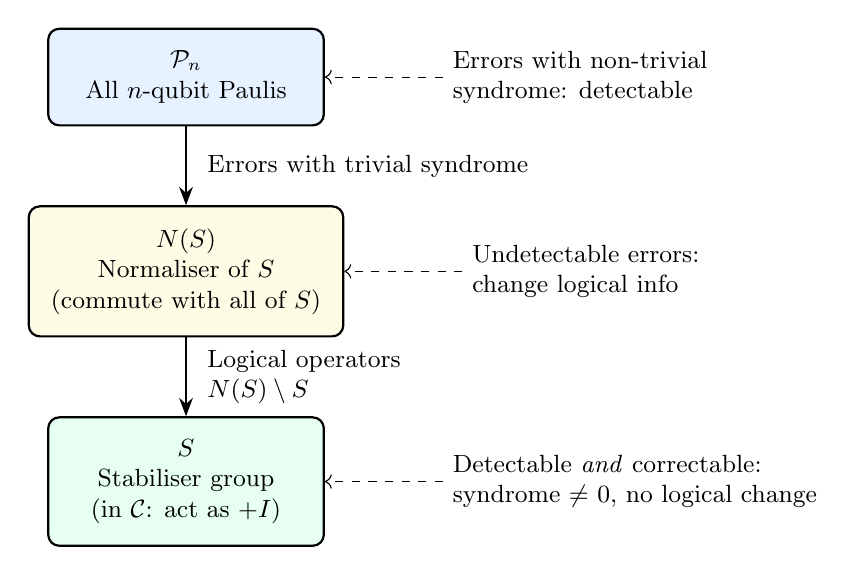
\begin{tikzpicture}[
  every node/.style={font=\small},
  box/.style={rectangle, rounded corners=4pt, draw, thick, inner sep=8pt,
              align=center, minimum width=3.5cm}
]
  \node[box, fill=lightblue, align=center]  (Pn) at (0,0)
    {$\mathcal{P}_n$ \\ All $n$-qubit Paulis};
  \node[box, fill=lightyellow, align=center, below=1cm of Pn]  (NS)
    {$N(S)$ \\ Normaliser of $S$ \\ (commute with all of $S$)};
  \node[box, fill=lightgreen, align=center, below=1cm of NS] (S)
    {$S$ \\ Stabiliser group \\ (in $\mathcal{C}$: act as $+I$)};

  \draw[-{Stealth}, thick] (Pn.south) -- (NS.north)
    node[midway, right=4pt, align=left] {Errors with trivial syndrome};
  \draw[-{Stealth}, thick] (NS.south) -- (S.north)
    node[midway, right=4pt, align=left] {Logical operators \\ $N(S)\setminus S$};

  \node[right=1.5cm of Pn, align=left, font=\small] (a)
    {Errors with non-trivial \\ syndrome: detectable};
  \draw[->, dashed] (a.west) -- (Pn.east);

  \node[right=1.5cm of NS, align=left, font=\small] (b)
    {Undetectable errors: \\ change logical info};
  \draw[->, dashed] (b.west) -- (NS.east);

  \node[right=1.5cm of S, align=left, font=\small] (c)
    {Detectable \emph{and} correctable: \\ syndrome $\neq$ 0, no logical change};
  \draw[->, dashed] (c.west) -- (S.east);
\end{tikzpicture}
\caption{Hierarchy of the Pauli group relative to the stabiliser $S$.
Errors in $\mathcal{P}_n \setminus N(S)$ are detectable; errors in
$N(S) \setminus S$ are logical operators (undetectable and harmful); errors
in $S$ act trivially.}
\label{fig:stabilizer-hierarchy}
\end{figure}

\begin{exercise}
For the 3-qubit bit-flip code, show that $X_1 X_2 X_3 \in N(S) \setminus S$
and that it acts as the logical $\bar{X}$ operator.
\end{exercise}

\begin{exercise}
Verify the KL conditions for the 3-qubit bit-flip code for the pair
$E_a = X_1$, $E_b = X_1$ (the ``diagonal'' case $a = b$).
\end{exercise}

\begin{exercise}
Show that the Steane code satisfies the KL conditions for single-qubit
$Z$-errors by checking that $\Pi Z_i^\dagger Z_j \Pi = 0$ for $i \neq j$
and $\Pi Z_i^2 \Pi = \Pi$ for any qubit $i$.
\end{exercise}

\begin{summarybox}
\textbf{Section 6 key points:}
\begin{itemize}
  \item A stabilizer code is defined by an abelian Pauli subgroup $S$; the
        code space is the $+1$ eigenspace of all generators.
  \item $n$ physical qubits, $n-k$ generators $\Rightarrow$ $k$ logical qubits.
  \item Syndrome measurement projects errors onto Pauli components without
        disturbing logical information.
  \item KL conditions: a code corrects error set $\{E_a\}$ iff projected
        error products are proportional to the code projector.
  \item Undetectable errors ($N(S)\setminus S$) act as logical operators;
        their minimum weight is the code distance $d$.
\end{itemize}
\end{summarybox}

% ======================================================================
% SECTION 7: SURFACE CODE
% ======================================================================
\newpage
\section{The Surface Code}
\label{sec:surface}

\begin{intuition}
The surface code is the most promising candidate for practical quantum
computers.  Imagine a checkerboard.  Data qubits sit on the \emph{edges} of
the board (the lines between squares).  Two kinds of stabilizers sit on the
squares themselves: ``plaquette'' stabilizers (on dark squares) measure $Z$
parities and detect $X$ errors; ``vertex'' stabilizers (on light squares)
measure $X$ parities and detect $Z$ errors.  An error creates a pair of
``defects'' on adjacent squares --- like flipping two squares on the
checkerboard --- and correcting the error means pairing up defects and erasing
them.
\end{intuition}

\subsection{Lattice Structure}

Consider a $d \times d$ square lattice where $d$ is the \textbf{code distance}:

\begin{itemize}
  \item \textbf{Data qubits} sit on the edges of the lattice (horizontal
        and vertical lines between vertices).
  \item \textbf{Z-stabilizers (plaquettes):} Each interior face of the lattice
        has a 4-qubit $Z$ stabilizer $Z_{e_1}Z_{e_2}Z_{e_3}Z_{e_4}$, where
        $e_1, \ldots, e_4$ are the four edges bounding that face.
  \item \textbf{X-stabilizers (vertices):} Each interior vertex has a 4-qubit
        $X$ stabilizer $X_{e_1}X_{e_2}X_{e_3}X_{e_4}$, where the edges are
        the four incident edges.
  \item Boundary qubits participate in 2- or 3-qubit stabilizers.
\end{itemize}

\subsubsection{Counting for a $d=3$ Surface Code}

For $d = 3$, the lattice has $d^2 + (d-1)^2 = 9 + 4 = 13$ data qubits.

\begin{figure}[H]
\centering
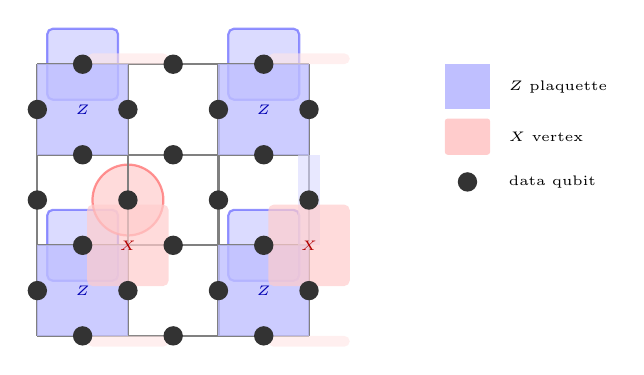
\begin{tikzpicture}[
  scale=1.15,
  qubit/.style={circle, fill=black!80, minimum size=7pt, inner sep=0pt},
  zstab/.style={rectangle, fill=blue!20, draw=blue!60, thick,
                minimum size=0.9cm, rounded corners=2pt, opacity=0.7},
  xstab/.style={circle, fill=red!20, draw=red!60, thick,
                minimum size=0.9cm, opacity=0.7},
  lbl/.style={font=\scriptsize}
]
  % Draw Z-stabilizer faces (plaquettes) - 4 of them for d=3
  \foreach \r/\c in {0/0, 0/2, 2/0, 2/2}{
    \node[zstab] at (\c+0.5, \r+0.5+0.5) {};
  }
  % Draw X-stabilizer vertices - interior ones
  \foreach \r/\c in {1/1}{
    \node[xstab] at (\c, \r+0.5) {};
  }
  % Actually let's draw a proper d=3 lattice
  % Grid lines (lattice edges = data qubits)
  % Horizontal edges
  \foreach \row in {0,1,2,3}{
    \foreach \col in {0,1,2}{
      \draw[thick, gray] (\col, \row) -- (\col+1, \row);
    }
  }
  % Vertical edges
  \foreach \row in {0,1,2}{
    \foreach \col in {0,1,2,3}{
      \draw[thick, gray] (\col, \row) -- (\col, \row+1);
    }
  }

  % Z-stabilizer plaquettes (faces), color them blue
  \foreach \row/\col in {0/0, 0/2, 2/0, 2/2}{
    \fill[blue!25, opacity=0.8] (\col,\row) rectangle (\col+1,\row+1);
    \node[font=\tiny, blue!70!black] at (\col+0.5, \row+0.5) {$Z$};
  }
  % Partial Z-stabilizers on boundary (2-qubit)
  \foreach \row/\col in {1/3}{
    \fill[blue!15, opacity=0.6] (\col-0.12, \row)
      rectangle (\col+0.12, \row+1);
    \node[font=\tiny, blue!60!black] at (\col, \row+0.5) {$Z$};
  }

  % X-stabilizer vertices (stars), color them red
  \foreach \row/\col in {0/1, 0/3, 2/1, 2/3}{
    % boundary
  }
  \foreach \row/\col in {1/1, 1/3}{
    \fill[red!20, opacity=0.7, rounded corners=2pt]
      (\col-0.45, \row-0.45) rectangle (\col+0.45, \row+0.45);
    \node[font=\tiny, red!70!black] at (\col, \row) {$X$};
  }
  % Half X on top/bottom boundary
  \foreach \col in {1,3}{
    \fill[red!10, opacity=0.6, rounded corners=2pt]
      (\col-0.45,3) rectangle (\col+0.45, 3.12);
    \fill[red!10, opacity=0.6, rounded corners=2pt]
      (\col-0.45,-0.12) rectangle (\col+0.45, 0);
  }

  % Data qubits on edges
  % Horizontal edges - midpoints
  \foreach \row in {0,1,2,3}{
    \foreach \col in {0,1,2}{
      \node[qubit] at (\col+0.5, \row) {};
    }
  }
  % Vertical edges - midpoints
  \foreach \row in {0,1,2}{
    \foreach \col in {0,1,2,3}{
      \node[qubit] at (\col, \row+0.5) {};
    }
  }

  % Legend
  \fill[blue!25] (4.5, 2.5) rectangle (5.0, 3.0);
  \node[right, font=\tiny] at (5.1, 2.75) {$Z$ plaquette};
  \fill[red!20, rounded corners=1pt] (4.5, 2.0) rectangle (5.0, 2.4);
  \node[right, font=\tiny] at (5.1, 2.2) {$X$ vertex};
  \node[qubit] at (4.75, 1.7) {};
  \node[right, font=\tiny] at (5.1, 1.7) {data qubit};
\end{tikzpicture}
\caption{A $d=3$ surface code lattice (schematic).  Black dots are data
qubits on edges.  Blue squares are $Z$-stabilizer plaquettes; red regions
are $X$-stabilizer vertices.  This encodes 1 logical qubit in 13 data qubits
with distance 3.}
\label{fig:surface-code-lattice}
\end{figure}

\subsubsection{Code Parameters}

For distance $d$:
\begin{align}
  \text{Data qubits: } n &= d^2 + (d-1)^2 = 2d^2 - 2d + 1 \label{eq:surface-n}\\
  \text{Z-stabilizers: } &(d-1)^2 + (d-1) = d(d-1) \\
  \text{X-stabilizers: } &d(d-1)\\
  \text{Logical qubits: } k &= 1 \quad\text{(for planar surface code)}\\
  \text{Code distance: } &d \quad\text{(minimum weight logical operator)}
\end{align}

\begin{workedexample}[Parameters for $d = 5$]
\[
  n = 2(25) - 10 + 1 = 41 \text{ data qubits.}
\]
Number of $Z$-stabilizers: $5\times4 = 20$.\\
Number of $X$-stabilizers: $5\times4 = 20$.\\
Total stabilizer measurements: $20 + 20 = 40$.\\
Logical qubits: $41 - 40 = 1$. \checkmark\\
Code distance: $d = 5$, so we can correct up to
$\lfloor(5-1)/2\rfloor = 2$ errors.
\end{workedexample}

\subsection{Error Correction: Minimum-Weight Perfect Matching}

\paragraph{How errors create syndromes.}
A chain of $X$-errors on a sequence of data qubits creates \emph{defects}
(syndrome $-1$ outcomes) at the \emph{endpoints} of the chain.

\begin{figure}[H]
\centering
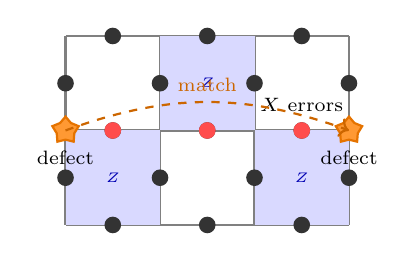
\begin{tikzpicture}[scale=1.2,
  qubit/.style={circle, fill=black!80, minimum size=6pt, inner sep=0pt},
  defect/.style={star, star points=5, fill=orange!80, draw=orange!90!black,
                 thick, minimum size=10pt, inner sep=0pt},
  xerr/.style={circle, fill=red!70, minimum size=6pt, inner sep=0pt}
]
  % 2x3 portion of lattice, simplified
  \draw[thick, gray] (0,0) grid (3,2);
  % Z-plaquettes
  \foreach \r/\c in {0/0, 0/2, 1/1}{
    \fill[blue!15] (\c,\r) rectangle (\c+1,\r+1);
    \node[font=\tiny, blue!70!black] at (\c+0.5,\r+0.5) {$Z$};
  }
  % Data qubits
  \foreach \r in {0,1,2}{ \foreach \c in {0,1,2}{
    \node[qubit] at (\c+0.5,\r) {};
  }}
  \foreach \r in {0,1}{ \foreach \c in {0,1,2,3}{
    \node[qubit] at (\c,\r+0.5) {};
  }}

  % X error chain on horizontal row y=1
  \node[xerr] at (0.5,1) {};
  \node[xerr] at (1.5,1) {};
  \node[xerr, label=above:{\scriptsize $X$ errors}] at (2.5,1) {};

  % Defects at endpoints
  \node[defect, label=below:{\scriptsize defect}] at (0,1) {};
  \node[defect, label=below:{\scriptsize defect}] at (3,1) {};

  % Arrow
  \draw[->, thick, orange!80!black, dashed] (0,1) to[bend left=20]
    node[above, font=\scriptsize]{match} (3,1);
\end{tikzpicture}
\caption{A chain of $X$-errors (red dots) on three data qubits creates
\emph{defects} (orange stars) only at the endpoints.  The MWPM algorithm
pairs up defects and infers the most likely error chain.}
\label{fig:surface-mwpm}
\end{figure}

\paragraph{Minimum-weight perfect matching (MWPM).}
\begin{enumerate}
  \item Measure all stabilizers; collect the positions of defects ($-1$
        outcomes).
  \item Defects come in pairs (by the topology of the lattice).
  \item Find the \textbf{minimum-weight perfect matching} --- pair up defects
        so that the total number of data qubits inferred to have errors is
        minimised (using the Blossom algorithm or similar).
  \item Apply the inferred correction.
\end{enumerate}

\subsection{Fault-Tolerance Threshold}

\begin{theorem}[Surface code threshold]
For the surface code under depolarising noise with error rate $p$ per gate:
\[
  p_L \propto \left(\frac{p}{p_{\rm th}}\right)^{\lfloor(d+1)/2\rfloor},
\]
where $p_{\rm th} \approx 1\%$ for standard depolarising noise.  The logical
error rate decreases \textbf{exponentially} with code distance $d$ provided
$p < p_{\rm th}$.
\end{theorem}

\begin{workedexample}[Logical error rate for $d=5$]
Take $p = 0.005$ (0.5\%) and $p_{\rm th} = 0.01$ (1\%).  Then
$p/p_{\rm th} = 0.5$ and:
\[
  p_L \propto (0.5)^{\lfloor 6/2 \rfloor} = (0.5)^3 = 0.125.
\]
For $d=7$: $p_L \propto (0.5)^4 = 0.0625$ --- a factor 2 improvement
per distance step.  For $d=11$: $(0.5)^6 \approx 0.016$.  This shows
why large distance (and thus many physical qubits) are needed to reach
extremely low logical error rates.
\end{workedexample}

\subsection{Logical Gates via Lattice Surgery}

Direct transversal gates on the surface code are limited.  Logical operations
are instead performed by \textbf{lattice surgery}:

\begin{description}
  \item[Logical CNOT:] Merge two code patches (measuring joint stabilizers
        along the interface), perform joint measurements, then split.
  \item[Logical Hadamard:] On the \emph{rotated} surface code (a
        $45^\circ$-rotated lattice), $H^{\otimes n}$ implements $\bar{H}$.
  \item[Logical $T$ gate:] Requires magic state distillation
        (Section~\ref{sec:magic}).
\end{description}

\begin{figure}[H]
\centering
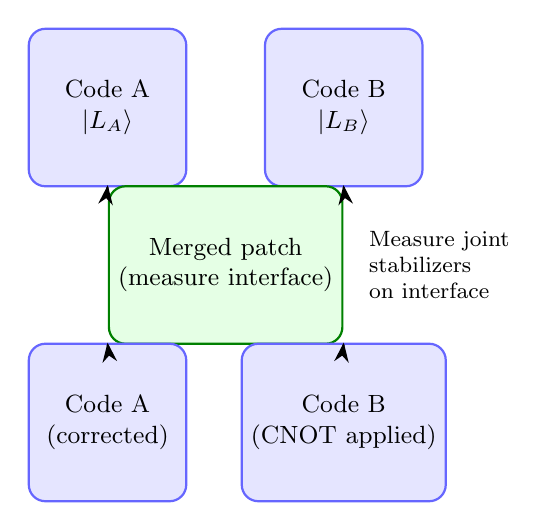
\begin{tikzpicture}[
  patch/.style={rectangle, rounded corners=6pt, draw=blue!60, thick,
                fill=blue!10, minimum width=2cm, minimum height=2cm,
                align=center, font=\small},
  arr/.style={-{Stealth[length=7pt]}, thick}
]
  \node[patch] (A) at (0,0) {Code A\\$\ket{L_A}$};
  \node[patch] (B) at (3,0) {Code B\\$\ket{L_B}$};
  \node[patch, fill=green!10, draw=green!50!black] (merged) at (1.5,-2)
    {Merged patch\\(measure interface)};
  \node[patch] (A2) at (0,-4) {Code A\\(corrected)};
  \node[patch] (B2) at (3,-4) {Code B\\(CNOT applied)};

  \draw[arr] (A.south) -- (merged.north west);
  \draw[arr] (B.south) -- (merged.north east);
  \draw[arr] (merged.south west) -- (A2.north);
  \draw[arr] (merged.south east) -- (B2.north);

  \node[right=0.2cm of merged, align=left, font=\footnotesize]
    {Measure joint\\stabilizers\\on interface};
\end{tikzpicture}
\caption{Lattice surgery for a logical CNOT.  Two code patches are
temporarily merged by measuring joint stabilizers on the interface, then
split again.  The net effect is a logical CNOT between qubits $A$ and $B$.}
\label{fig:lattice-surgery}
\end{figure}

\subsection{Why the Surface Code is Practical}

\begin{itemize}
  \item \textbf{Local interactions only:} Each stabilizer involves at most
        4 nearest-neighbour qubits --- perfectly suited to 2D chip architectures
        (superconducting qubits, trapped ions arranged in a plane).
  \item \textbf{High threshold:} $p_{\rm th} \approx 1\%$ is achievable with
        current hardware ($p \sim 0.1$--$0.5\%$).
  \item \textbf{Simple decoding:} MWPM is efficient (polynomial time).
  \item \textbf{Natural fault-tolerance:} Stabilizer measurement errors can
        be tracked across repeated measurement rounds.
\end{itemize}

\begin{exercise}
Calculate the number of data qubits, $Z$-stabilizers, $X$-stabilizers, and
logical qubits for a $d=7$ surface code.  Verify $k=1$.
\end{exercise}

\begin{exercise}
A chain of two $X$-errors occurs on adjacent data qubits in a $d=3$ surface
code.  Draw the defect pattern and explain how MWPM would (correctly) decode
this error.  Now suppose three consecutive $X$-errors form a chain spanning
the lattice.  Why does this cause a logical error?
\end{exercise}

\begin{exercise}
Below the threshold, the logical error rate scales as
$p_L \propto (p/p_{\rm th})^{(d+1)/2}$.  How large must $d$ be to achieve
$p_L < 10^{-10}$ if $p = 0.003$ and $p_{\rm th} = 0.01$?
\end{exercise}

\begin{summarybox}
\textbf{Section 7 key points:}
\begin{itemize}
  \item The surface code places data qubits on lattice edges; $Z$ (plaquette)
        and $X$ (vertex) stabilizers detect bit- and phase-flip errors.
  \item A $d=d$ surface code uses $2d^2-2d+1$ qubits, has distance $d$,
        and encodes 1 logical qubit.
  \item Errors create defect pairs; MWPM corrects by pairing defects
        optimally.
  \item Threshold $p_{\rm th} \approx 1\%$; logical error rate drops
        exponentially with $d$ below threshold.
  \item Logical gates via lattice surgery; $T$ gate still requires magic
        state distillation.
\end{itemize}
\end{summarybox}

% ======================================================================
% SECTION 8: FAULT-TOLERANT GATES
% ======================================================================
\newpage
\section{Fault-Tolerant Quantum Gates}
\label{sec:fault-tolerant}

\begin{intuition}
Encoding qubits protects stored information, but we also need to
\emph{compute} on it.  A gate performed directly on physical qubits might
spread a single error into many errors --- too many for the code to correct.
Fault-tolerant gate design is the art of performing logical operations in
a way that guarantees a single physical fault produces at most one logical
fault.
\end{intuition}

\subsection{Why Naive Gate Application Fails}

Consider applying a transversal CNOT to the 3-qubit bit-flip code.  A single
fault in the gate could spread to affect multiple qubits.  Suppose the second
CNOT gate has an $X$ error on its control:

\begin{figure}[H]
\centering
\begin{quantikz}[row sep=0.4cm]
  \lstick{$q_1$} & \ctrl{1} & \ctrl{2} & \qw\\
  \lstick{$q_2$} & \targ{}  & \qw & \qw\\
  \lstick{$q_3$} & \qw & \targ{} & \qw
\end{quantikz}
\quad$\to$\quad
\begin{quantikz}[row sep=0.4cm]
  \lstick{$q_1$} & \gate{X_{\rm err}} & \ctrl{1} & \ctrl{2} & \qw\\
  \lstick{$q_2$} & \qw & \targ{} & \qw & \qw\\
  \lstick{$q_3$} & \qw & \qw & \targ{} & \qw
\end{quantikz}
\caption{A single error on the first gate in the encoding circuit propagates
to affect all subsequent qubits.  This ``error spreading'' is the key danger
that fault-tolerant design must prevent.}
\end{figure}

\subsection{Transversal Gates}

\begin{definition}[Transversal gate]
A gate $U_L$ is \textbf{transversal} if it can be written as
$U_L = u^{\otimes n}$ (same single-qubit operation on every physical qubit,
possibly with qubit permutations between code blocks).
\end{definition}

A transversal gate is automatically fault-tolerant: a fault on physical
qubit $j$ affects only qubit $j$ in the encoded block --- it cannot spread to
other qubits.

\begin{center}
\renewcommand{\arraystretch}{1.4}
\begin{tabular}{@{} l l l @{}}
  \toprule
  \textbf{Code} & \textbf{Transversal gates} & \textbf{Missing gates}\\
  \midrule
  3-qubit bit-flip & $\overline{X}$, $\overline{Z}$ & Phase, $T$, Hadamard\\
  Steane $\code{7,1,3}$ & $\bar{H}$, $\bar{S}$, $\overline{\text{CNOT}}$
    (Clifford group) & $T$ gate\\
  Surface code & $\bar{H}$ (rotated), $\overline{\text{CNOT}}$ via surgery
    & $T$ gate\\
  \bottomrule
\end{tabular}
\end{center}

\begin{theorem}[Eastin--Knill theorem]
No quantum error-correcting code can have a transversal implementation of
a \textbf{universal} gate set.
\end{theorem}

This means every code must use some non-transversal technique for at least
one gate.  The $T$ gate ($\pi/8$ gate) is the standard choice.

\subsection{Fault-Tolerant Syndrome Measurement}

Measuring a multi-qubit stabilizer like $Z_1 Z_2 Z_3 Z_4$ requires ancilla
qubits.  A naive circuit might look like:

\begin{figure}[H]
\centering
\begin{quantikz}[row sep=0.4cm, column sep=0.5cm]
  \lstick{$q_1$} & \ctrl{4} & \qw & \qw & \qw & \qw\\
  \lstick{$q_2$} & \qw & \ctrl{3} & \qw & \qw & \qw\\
  \lstick{$q_3$} & \qw & \qw & \ctrl{2} & \qw & \qw\\
  \lstick{$q_4$} & \qw & \qw & \qw & \ctrl{1} & \qw\\
  \lstick{$\ket{0}$} & \targ{} & \targ{} & \targ{} & \targ{} & \meter{$s$}
\end{quantikz}
\caption{Standard ancilla-based syndrome measurement for the $Z_1Z_2Z_3Z_4$
stabilizer.  The ancilla records the parity of the four data qubits.
One fault in this circuit can propagate to multiple data qubits.}
\label{fig:syndrome-circuit}
\end{figure}

\begin{caution}
A single fault in the ancilla preparation or the CNOT gates can spread to
multiple data qubits.  For example, an $X$ error on the ancilla before any
CNOT will propagate a $Z$ error to \emph{every} data qubit it interacts with
(since $Z$ errors on the target propagate to the control).  This can defeat
the code's error-correcting power.  The solution is to use
\textbf{flag qubits} or \textbf{cat states} to detect such spreading.
\end{caution}

\subsubsection{Repeated Measurement}

Even with perfect gates, measurement outcomes themselves are noisy.  The
standard approach is to repeat stabilizer measurements (typically 3 times
for a distance-3 code) and use the majority outcome or track the syndrome
history.  For the surface code, syndrome measurements are repeated $O(d)$
times to reliably decode.

\subsection{Magic State Distillation}
\label{sec:magic}

\subsubsection{Why We Need Magic States}

We need a universal gate set.  The Clifford gates (which include $H$, $S$,
CNOT) are transversal in many codes, but they are \emph{not} universal: any
circuit built from Clifford gates alone can be simulated classically in
polynomial time (Gottesman--Knill theorem).

To achieve universality, we add the $T$ gate:
\[
  T = \begin{pmatrix}1 & 0\\ 0 & e^{i\pi/4}\end{pmatrix}.
\]
The Clifford group plus $T$ is universal.  However, $T$ is not transversal
in standard codes.

\subsubsection{The Magic State Idea}

The $T$ gate can be implemented by \textbf{gate teleportation} if we have
access to the \textbf{magic state}:
\[
  \ket{T} = T\ket{+} = \frac{\ket{0} + e^{i\pi/4}\ket{1}}{\sqrt{2}}.
\]

The teleportation circuit uses only Clifford gates plus a measurement:

\begin{figure}[H]
\centering
\begin{quantikz}[row sep=0.5cm, column sep=0.6cm]
  \lstick{$\ket{\psi}$} & \ctrl{1} & \gate{S^{m}} & \qw
    & \rstick{$T\ket{\psi}$}\\
  \lstick{$\ket{T}$}    & \targ{}  & \meter{$m$}  &
\end{quantikz}
\caption{Gate teleportation implementing the $T$ gate.  Given one copy of the
magic state $\ket{T}$, a Clifford correction $S^m$ (where $m \in \{0,1\}$
is the measurement result) yields $T\ket{\psi}$ using only Clifford gates.}
\label{fig:gate-teleportation}
\end{figure}

\subsubsection{Distillation Protocol}

Physical $T$ gates are noisy; the resulting states are close to
(but not exactly) $\ket{T}$.  The \textbf{15-to-1 distillation protocol}
(Bravyi--Kitaev) takes 15 noisy magic states and produces 1 high-fidelity
magic state:

\begin{itemize}
  \item Input: 15 noisy $\ket{T}$ states, each with error probability $\epsilon$.
  \item Output: 1 magic state with error probability
        $\approx 35\epsilon^3$ (superquadratic suppression).
  \item Circuit: uses only Clifford gates (which are fault-tolerant
        transversally) to distil the high-quality state.
\end{itemize}

\begin{workedexample}[Distillation improvement]
If the physical $T$ gate has error rate $\epsilon = 0.01$:
\begin{align*}
  \text{After 1 round: } &\epsilon_1 \approx 35(0.01)^3 = 35 \times 10^{-6}
    = 3.5 \times 10^{-5}.\\
  \text{After 2 rounds: } &\epsilon_2 \approx 35(3.5\times10^{-5})^3
    \approx 1.5 \times 10^{-12}.
\end{align*}
Two rounds of 15-to-1 distillation reduce the error from 1\% to below
$10^{-12}$ at the cost of $15^2 = 225$ initial magic states.
\end{workedexample}

\subsection{The Threshold Theorem}
\label{sec:threshold}

\begin{theorem}[Fault-Tolerant Threshold Theorem]
\label{thm:threshold}
Suppose each physical gate, preparation, and measurement has error rate
$p$, and errors are local (independent across qubits).  There exists a
threshold $p_{\rm th} > 0$ such that: if $p < p_{\rm th}$, arbitrarily long
quantum computations can be performed with failure probability approaching 0.
The qubit overhead scales as $\text{poly}(\log(1/\epsilon))$ for target
error $\epsilon$.
\end{theorem}

\begin{itemize}
  \item For the surface code: $p_{\rm th} \approx 1\%$ (depolarising noise).
  \item For concatenated codes (Section~\ref{sec:advanced}):
        $p_{\rm th} \approx 10^{-4}$ to $10^{-3}$.
  \item The surface code's higher threshold is a major reason it is the
        leading practical candidate.
\end{itemize}

\subsubsection{Below vs.\ Above Threshold}

\begin{figure}[H]
\centering
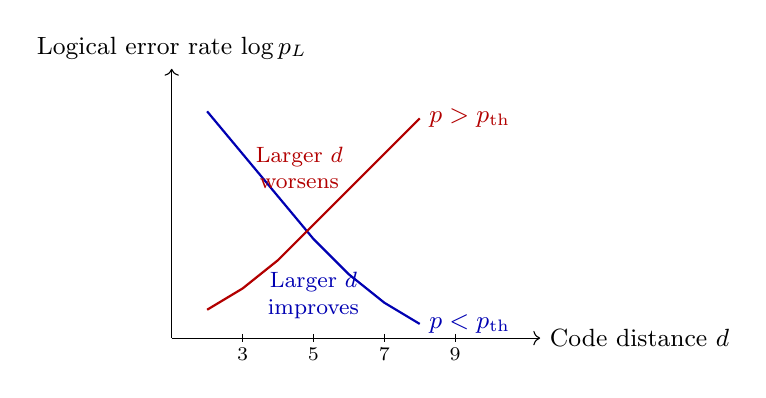
\begin{tikzpicture}[scale=0.9]
  \draw[->] (0,0) -- (5.2,0) node[right, font=\small] {Code distance $d$};
  \draw[->] (0,0) -- (0,3.8) node[above, font=\small] {Logical error rate $\log p_L$};
  % Below threshold line (decreasing)
  \draw[thick, blue!70!black]
    (0.5, 3.2) -- (1.0, 2.6) -- (1.5, 2.0) -- (2.0, 1.4)
    -- (2.5, 0.9) -- (3.0, 0.5) -- (3.5, 0.2);
  \node[right, font=\small, blue!70!black] at (3.5, 0.2) {$p < p_{\rm th}$};
  % Above threshold line (increasing)
  \draw[thick, red!70!black]
    (0.5, 0.4) -- (1.0, 0.7) -- (1.5, 1.1) -- (2.0, 1.6)
    -- (2.5, 2.1) -- (3.0, 2.6) -- (3.5, 3.1);
  \node[right, font=\small, red!70!black] at (3.5, 3.1) {$p > p_{\rm th}$};
  % Labels
  \node[font=\footnotesize, blue!70!black, align=center] at (2.0, 0.6)
    {Larger $d$\\improves};
  \node[font=\footnotesize, red!70!black, align=center] at (1.8, 2.4)
    {Larger $d$\\worsens};
  % Tick marks
  \foreach \x/\lbl in {1/3, 2/5, 3/7, 4/9}{
    \draw (\x, 0.06) -- (\x, -0.06);
    \node[below, font=\scriptsize] at (\x, 0) {$\lbl$};
  }
\end{tikzpicture}
\caption{Below the threshold (blue), increasing code distance decreases the
logical error rate exponentially.  Above the threshold (red), adding more
qubits makes things worse because there are too many opportunities for error.}
\label{fig:threshold}
\end{figure}

\begin{exercise}
For a $d=7$ surface code with $p = 0.004$ and $p_{\rm th} = 0.01$, estimate
the logical error rate as a multiple of $(p/p_{\rm th})^{\lfloor(d+1)/2\rfloor}$.
\end{exercise}

\begin{exercise}
Using the gate teleportation circuit of Figure~\ref{fig:gate-teleportation},
verify that measuring the ancilla in state $\ket{1}$ (outcome $m=1$) and
then applying $S$ to the data qubit produces $T\ket{\psi}$.
(\emph{Hint:} work through the action of the CNOT on $\ket{\psi}\ket{T}$,
then project onto $m=0$ and $m=1$ separately.)
\end{exercise}

\begin{exercise}
After three levels of 15-to-1 distillation starting from $\epsilon = 0.005$,
what is the estimated output magic state error rate?  How many physical
$T$-gate preparations does this require?
\end{exercise}

\begin{summarybox}
\textbf{Section 8 key points:}
\begin{itemize}
  \item Transversal gates prevent error spreading; the Eastin--Knill theorem
        says no code has a universal transversal gate set.
  \item Syndrome measurement circuits must be designed carefully to avoid
        fault propagation; repeated measurement is needed.
  \item The $T$ gate is implemented via gate teleportation using magic states.
  \item Magic state distillation (15-to-1 protocol) converts many noisy
        $\ket{T}$ states into one high-fidelity one.
  \item The threshold theorem guarantees scalable quantum computation when
        physical error rates are below $p_{\rm th}$.
\end{itemize}
\end{summarybox}

% ======================================================================
% SECTION 9: ADVANCED TOPICS
% ======================================================================
\newpage
\section{Advanced Topics in Quantum Error Correction}
\label{sec:advanced}

\begin{intuition}
The surface code is excellent but has one major weakness: it encodes only
1 logical qubit no matter how many physical qubits you use.  For a practical
quantum computer running a million-gate algorithm, you might need thousands
of logical qubits, requiring millions of physical qubits.  This section
surveys alternative codes that offer better rates (more logical qubits per
physical qubit), higher thresholds, or additional transversal gates.
\end{intuition}

\subsection{Quantum Low-Density Parity-Check (LDPC) Codes}

Classical LDPC codes are a major tool in classical communications (used in
5G, WiFi, etc.).  Each parity-check involves few bits (\textbf{sparse}) and
each bit appears in few checks --- hence ``low density''.

Quantum LDPC codes generalise this to the stabilizer setting:
\begin{itemize}
  \item Each stabilizer generator involves at most $w$ qubits (for some
        constant $w$, e.g.\ $w=6$).
  \item Each qubit appears in at most $w$ generators.
  \item Result: sparse syndrome measurement circuits, fewer gates per round.
\end{itemize}

\subsubsection{Recent Breakthrough: Good Quantum LDPC Codes}

\begin{center}
\renewcommand{\arraystretch}{1.3}
\begin{tabular}{@{} l c c c @{}}
  \toprule
  \textbf{Code family} & \textbf{Rate $k/n$} & \textbf{Distance $d$}
    & \textbf{Stabilizer weight}\\
  \midrule
  Surface code & $\Theta(1/n)$ & $\Theta(\sqrt{n})$ & 4\\
  Hypergraph product & Constant & $\Theta(\sqrt{n})$ & $O(1)$\\
  Lifted product (Panteleev--Kalachev 2022) & Constant & $\Theta(n)$ & $O(1)$\\
  Fiber bundle codes & Constant & $\Theta(n^{3/5})$ & $O(1)$\\
  \bottomrule
\end{tabular}
\end{center}

A code with \emph{constant rate} and \emph{linear distance} ($d = \Theta(n)$)
is called a \textbf{good quantum LDPC code}.  These were only proved to exist
in 2022, representing a major theoretical advance.

\subsubsection{Practical Challenges}

Despite better parameters, quantum LDPC codes face challenges:
\begin{itemize}
  \item Generators can involve non-local (long-range) qubit pairs --- hard
        to implement in 2D architectures.
  \item Efficient decoders are still being developed.
  \item Threshold values and exact overheads are not yet as well understood
        as for the surface code.
\end{itemize}

\subsection{Color Codes}

Color codes are topological codes defined on 3-colorable lattices.

\subsubsection{2D Color Code Construction}

Consider a 2D lattice where every face can be colored red, green, or blue,
and every vertex touches exactly one face of each color.  Data qubits sit on
the vertices.

\begin{figure}[H]
\centering
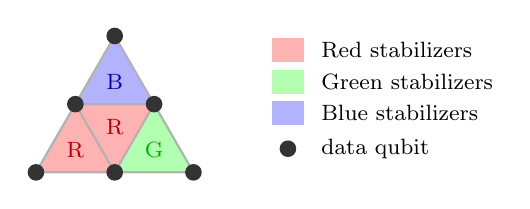
\begin{tikzpicture}[scale=1.0,
  qubit/.style={circle, fill=black!80, minimum size=6pt, inner sep=0pt},
  lbl/.style={font=\footnotesize}
]
  % Triangular lattice, 3-colorable
  % Red face
  \fill[red!30] (0,0) -- (1,0) -- (0.5, 0.866) -- cycle;
  \node[lbl, red!70!black] at (0.5, 0.29) {R};
  % Green face
  \fill[green!30] (1,0) -- (2,0) -- (1.5, 0.866) -- cycle;
  \node[lbl, green!70!black] at (1.5, 0.29) {G};
  % Blue face
  \fill[blue!30] (0.5, 0.866) -- (1.5, 0.866) -- (1, 1.732) -- cycle;
  \node[lbl, blue!70!black] at (1.0, 1.15) {B};
  % Red face 2
  \fill[red!30] (0.5, 0.866) -- (1,0) -- (1.5, 0.866) -- cycle;
  \node[lbl, red!70!black] at (1.0, 0.58) {R};

  % Edges
  \draw[thick, gray!60]
    (0,0) -- (1,0) -- (2,0)
    (0,0) -- (0.5, 0.866) -- (1,0)
    (1,0) -- (1.5, 0.866) -- (2,0)
    (0.5, 0.866) -- (1, 1.732) -- (1.5, 0.866)
    (0.5, 0.866) -- (1.5, 0.866);

  % Data qubits on vertices
  \foreach \x/\y in {0/0, 1/0, 2/0, 0.5/0.866, 1.5/0.866, 1/1.732}{
    \node[qubit] at (\x,\y) {};
  }

  % Legend
  \fill[red!30] (3, 1.4) rectangle (3.4, 1.7);
  \node[lbl, right] at (3.5, 1.55) {Red stabilizers};
  \fill[green!30] (3, 1.0) rectangle (3.4, 1.3);
  \node[lbl, right] at (3.5, 1.15) {Green stabilizers};
  \fill[blue!30] (3, 0.6) rectangle (3.4, 0.9);
  \node[lbl, right] at (3.5, 0.75) {Blue stabilizers};
  \node[qubit] at (3.2, 0.3) {};
  \node[lbl, right] at (3.5, 0.3) {data qubit};
\end{tikzpicture}
\caption{A small portion of a 2D color code lattice.  Each colored face
contributes both an $X$-type and a $Z$-type stabilizer on its vertices.
The 3-colorability allows fault-tolerant gates beyond those of the surface
code.}
\label{fig:color-code}
\end{figure}

For each colored face $f$, there is an $X$-stabilizer and a $Z$-stabilizer
on the vertices of $f$.  The code is a $\code{n,1,d}$ code similar to the
surface code.

\subsubsection{Advantages of Color Codes}

\begin{itemize}
  \item The 2D color code has the same parameters as the surface code
        ($d = \Theta(\sqrt{n})$, rate $1/n$) but admits
        \textbf{transversal} $H$, $S$, $\text{CNOT}$, \emph{and} $T$ in
        some 3D variants.
  \item In 3D color codes, the full Clifford$+T$ gate set is transversal,
        eliminating the need for magic state distillation --- though at the
        cost of a 3D qubit architecture.
  \item Syndrome extraction is slightly more complex than for the surface
        code.
\end{itemize}

\subsection{Concatenated Codes}

\begin{definition}[Code concatenation]
Given an ``outer'' code $C_1 = \code{n_1, k_1, d_1}$ and an ``inner'' code
$C_2 = \code{n_2, k_2, d_2}$ with $k_2 = k_1$, the
\textbf{concatenated code} $C_1 \circ C_2$ encodes each physical qubit
of $C_1$ using the inner code $C_2$.  The result is a
$\code{n_1 n_2, k_1, d_1 d_2}$ code.
\end{definition}

\begin{workedexample}[Concatenating two Steane codes]
Let both $C_1$ and $C_2$ be the Steane $\code{7,1,3}$ code.
The concatenated code $C_1 \circ C_2$ has:
\begin{align*}
  n &= 7 \times 7 = 49 \text{ physical qubits},\\
  k &= 1 \text{ logical qubit},\\
  d &= 3 \times 3 = 9.
\end{align*}
After $\ell$ levels of concatenation:
\[
  n_\ell = 7^\ell, \quad d_\ell = 3^\ell, \quad k = 1.
\]

\textbf{Logical error rate under concatenation:}
Let $p$ be the physical error rate.  After $\ell$ levels:
\[
  p_L^{(\ell)} \approx \frac{1}{c}\bigl(c\,p\bigr)^{2^\ell},
\]
where $c$ is a constant depending on the code (for Steane, $c \approx 1/p_{\rm th}$).
For $p = 0.001$ and $c = 100$:
\[
  \ell=1: \quad p_L \approx (0.1)^2 = 0.01.
\]
\[
  \ell=2: \quad p_L \approx (0.1)^4 = 10^{-4}.
\]
\[
  \ell=3: \quad p_L \approx (0.1)^8 = 10^{-8}.
\]
Exponential suppression, but at the cost of $7^3 = 343$ physical qubits per
logical qubit at level 3.
\end{workedexample}

\subsection{Comparison of QEC Code Families}

\begin{center}
\renewcommand{\arraystretch}{1.4}
\begin{tabular}{@{} l c c c c @{}}
  \toprule
  \textbf{Code} & \textbf{Rate} & \textbf{Distance} &
    \textbf{Transversal gates} & \textbf{Architecture}\\
  \midrule
  Surface & $\Theta(1/n)$ & $\Theta(\sqrt{n})$ & Clifford (partial) & 2D local\\
  Color (2D) & $\Theta(1/n)$ & $\Theta(\sqrt{n})$ & Full Clifford & 2D local\\
  Color (3D) & $\Theta(1/n)$ & $\Theta(n^{1/3})$ & Clifford + $T$ & 3D local\\
  Quantum LDPC & Constant & up to $\Theta(n)$ & Limited & Non-local\\
  Concatenated & Variable & Exponential & Depends & Non-local\\
  \bottomrule
\end{tabular}
\end{center}

\begin{exercise}
After 4 levels of concatenation with a $\code{7,1,3}$ code, how many
physical qubits encode 1 logical qubit?  What is the code distance?
\end{exercise}

\begin{exercise}
Explain why quantum LDPC codes with constant rate are important for practical
quantum computation.  What obstacles prevent their immediate use?
\end{exercise}

\begin{exercise}
A 2D color code and a surface code of the same physical qubit count $n$
both have distance $\Theta(\sqrt{n})$.  List two advantages of the color
code and one advantage of the surface code.
\end{exercise}

\begin{summarybox}
\textbf{Section 9 key points:}
\begin{itemize}
  \item Quantum LDPC codes offer constant rate (many logical qubits per
        physical qubit) with sparse stabilizers; recent breakthroughs
        achieve linear distance.
  \item Color codes are topological codes on 3-colorable lattices; 3D
        variants allow transversal $T$ gates.
  \item Concatenated codes reduce logical error rates doubly-exponentially
        in the number of concatenation levels, at exponential qubit cost.
  \item No single code is optimal for all metrics; the choice depends on
        hardware architecture, target error rate, and gate set requirements.
\end{itemize}
\end{summarybox}

% ======================================================================
% SECTION 10: SUMMARY
% ======================================================================
\newpage
\section{Summary and Putting It All Together}
\label{sec:summary}

This section brings together all the major themes of the course.

\subsection{The Big Picture}

Quantum error correction solves the fundamental problem of quantum
computation: qubits decohere and gates are imperfect.  The key ideas, in
order of development, are:

\begin{enumerate}
  \item \textbf{Errors are continuous, but correctable discretely.}
        Any single-qubit error decomposes into Pauli operators; syndrome
        measurement projects errors onto discrete Pauli faults.

  \item \textbf{Entanglement protects information.}
        Encoding in entangled states spreads information holographically
        across many qubits.  No individual qubit holds the secret.

  \item \textbf{Syndromes are the key.}
        Measuring stabilizers reveals errors without collapsing the
        logical superposition.  This is the central miracle of QEC.

  \item \textbf{Fault-tolerance requires more than encoding.}
        Gates, measurements, and state preparations must all be performed
        in ways that prevent single faults from cascading.

  \item \textbf{The threshold theorem gives hope.}
        Provided physical error rates are below $\sim 1\%$, reliable
        large-scale quantum computation is in principle possible.
\end{enumerate}

\subsection{Quick Reference: All Codes Covered}

\begin{center}
\renewcommand{\arraystretch}{1.5}
\begin{tabular}{@{} l c c c l @{}}
  \toprule
  \textbf{Code} & $n$ & $k$ & $d$ & \textbf{What it corrects}\\
  \midrule
  3-qubit bit-flip & 3 & 1 & 1 & Single $X$ error\\
  3-qubit phase-flip & 3 & 1 & 1 & Single $Z$ error\\
  Shor 9-qubit & 9 & 1 & 3 & Any single-qubit error\\
  Steane $\code{7,1,3}$ & 7 & 1 & 3 & Any single-qubit error\\
  Surface code ($d=5$) & 41 & 1 & 5 & Any 2-qubit error\\
  \bottomrule
\end{tabular}
\end{center}

\subsection{Road Map Through the Material}

\begin{figure}[H]
\centering
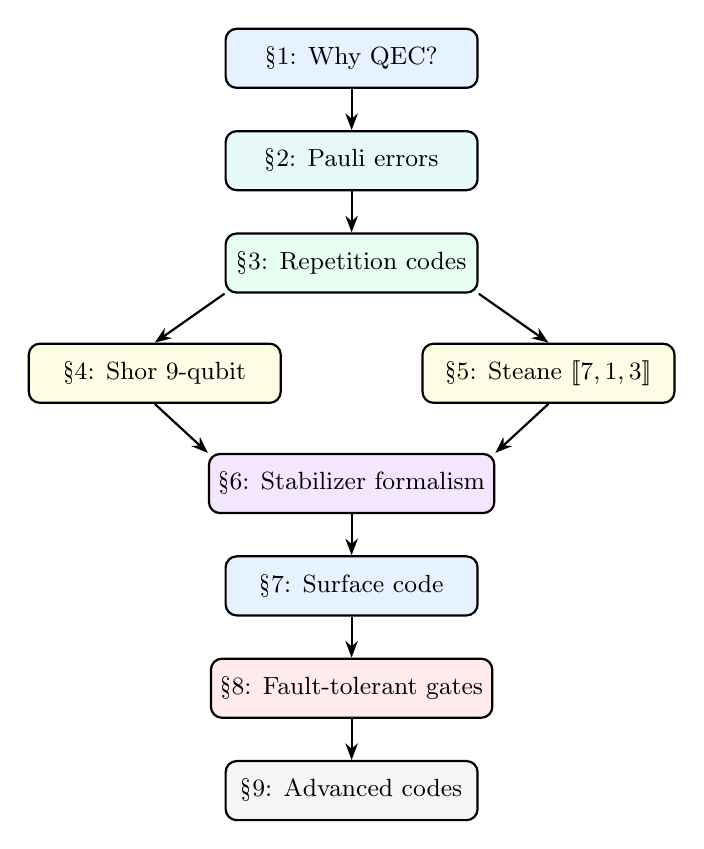
\begin{tikzpicture}[
  box/.style={rectangle, rounded corners=4pt, draw, thick,
              minimum width=3.2cm, minimum height=0.75cm,
              align=center, font=\small},
  arr/.style={-{Stealth[length=6pt]}, thick}
]
  \node[box, fill=lightblue]  (intro) at (0,0)   {\S1: Why QEC?};
  \node[box, fill=lightteal]  (pauli) at (0,-1.3) {\S2: Pauli errors};
  \node[box, fill=lightgreen] (rep)   at (0,-2.6) {\S3: Repetition codes};
  \node[box, fill=lightyellow](shor)  at (-2.5,-4.0) {\S4: Shor 9-qubit};
  \node[box, fill=lightyellow](steane)at (2.5,-4.0) {\S5: Steane $\code{7,1,3}$};
  \node[box, fill=lightpurple](stab)  at (0,-5.4) {\S6: Stabilizer formalism};
  \node[box, fill=lightblue]  (surf)  at (0,-6.7) {\S7: Surface code};
  \node[box, fill=lightred]   (ft)    at (0,-8.0) {\S8: Fault-tolerant gates};
  \node[box, fill=lightgray]  (adv)   at (0,-9.3) {\S9: Advanced codes};

  \draw[arr] (intro) -- (pauli);
  \draw[arr] (pauli) -- (rep);
  \draw[arr] (rep.south west) -- (shor.north);
  \draw[arr] (rep.south east) -- (steane.north);
  \draw[arr] (shor.south) -- (stab.north west);
  \draw[arr] (steane.south) -- (stab.north east);
  \draw[arr] (stab) -- (surf);
  \draw[arr] (surf) -- (ft);
  \draw[arr] (ft) -- (adv);
\end{tikzpicture}
\caption{The logical dependency structure of these lecture notes.  Each
section builds on the previous; Sections 4 and 5 are parallel examples that
Section 6 unifies.}
\end{figure}

\subsection{Comprehensive Exercises}

These exercises require combining knowledge from multiple sections.

\begin{exercise}
\textbf{[Full worked pipeline.]}
A logical qubit is encoded in the 3-qubit bit-flip code.
(a) Write the encoded state for $\ket{\psi} = \tfrac{1}{\sqrt{3}}\ket{0}
+ \sqrt{\tfrac{2}{3}}\ket{1}$.
(b) Suppose a $Y_2 = iX_2Z_2$ error occurs.  Compute the syndrome.
(c) Apply the corrective operation and verify the state is restored.
\end{exercise}

\begin{exercise}
\textbf{[KL conditions.]}
Prove that the Shor code satisfies the KL conditions for the error pair
$E_a = Z_1$ (phase flip on qubit 1) and $E_b = Z_4$ (phase flip on qubit 4).
\end{exercise}

\begin{exercise}
\textbf{[Code comparison.]}
For a quantum computer needing $p_L = 10^{-12}$ per logical gate with
physical error rate $p = 0.001$:
(a) How large must $d$ be for the surface code?
(b) How many levels of Steane code concatenation achieve this?
(c) Which uses fewer physical qubits?
\end{exercise}

\begin{exercise}
\textbf{[Steane code $X$-syndrome.]}
Suppose $Z$-errors occur on qubits 2 and 6 simultaneously in the Steane
code.  Compute the full $X$-syndrome and determine whether both errors
can be identified and corrected.
(\emph{Hint:} Check whether the combined syndrome is the XOR of the
individual syndromes.)
\end{exercise}

\begin{exercise}
\textbf{[Surface code threshold.]}
A surface code operates at $p = 0.008$ with $p_{\rm th} = 0.01$.
At what code distance $d$ does the logical error rate first drop below
$10^{-6}$?  How many physical qubits does this require?
\end{exercise}

\begin{exercise}
\textbf{[Magic state overhead.]}
A quantum algorithm requires $10^6$ $T$-gate applications.  Using the
15-to-1 distillation protocol with two rounds of distillation, and assuming
each logical Clifford gate consumes one magic state, how many physical
$T$-gate preparations are needed in total?
\end{exercise}

\begin{exercise}
\textbf{[Error channel.]}
A qubit undergoes a dephasing channel with $p = 0.1$, followed by a
bit-flip channel with $q = 0.05$.  Write the combined error channel as
a sum of Kraus operators and identify the probabilities of each Pauli error.
\end{exercise}

\begin{exercise}
\textbf{[Stabilizer design.]}
Design a simple 5-qubit code (the ``perfect code'' $\code{5,1,3}$) with
stabilizers $\{XZZXI, IXZZX, XIXZZ, ZXIXZ\}$ (where we write operators
on 5 qubits without tensor product symbols for brevity).
(a) Verify that all four generators commute.
(b) Show that the code encodes 1 logical qubit.
(c) Show that it has distance 3.
\end{exercise}

\begin{exercise}
\textbf{[Discretisation revisited.]}
A qubit suffers a general unitary error $U = \cos\theta\, I + i\sin\theta\, Z$
for $\theta = \pi/6$.  The qubit is protected by the 3-qubit phase-flip code.
(a) Decompose $U$ in the Pauli basis.
(b) After syndrome measurement, what is the probability that no correction
    is needed?  That a correction is applied?
(c) Verify that the final state is correct in both cases.
\end{exercise}

% ======================================================================
% BIBLIOGRAPHY
% ======================================================================
\newpage
\begin{thebibliography}{9}

\bibitem{nielsen2010}
Nielsen, M.~A.\ \& Chuang, I.~L.\ (2010).
\textit{Quantum Computation and Quantum Information: 10th Anniversary Edition}.
Cambridge University Press.
\textit{The standard reference.  Chapters 10--11 cover QEC and fault tolerance.}

\bibitem{shor1995}
Shor, P.~W.\ (1995).
Scheme for reducing decoherence in quantum computer memory.
\textit{Physical Review A}, 52(4), R2493.
\textit{The original 9-qubit code paper.}

\bibitem{steane1996}
Steane, A.~M.\ (1996).
Error correcting codes in quantum theory.
\textit{Physical Review Letters}, 77(5), 793.
\textit{The $\code{7,1,3}$ CSS code.}

\bibitem{knill1997}
Knill, E.\ \& Laflamme, R.\ (1997).
Theory of quantum error-correcting codes.
\textit{Physical Review A}, 55(2), 900.
\textit{The Knill--Laflamme error correction conditions.}

\bibitem{kitaev1997}
Kitaev, A.~Y.\ (1997).
Quantum computations: algorithms and error correction.
\textit{Russian Mathematical Surveys}, 52(6), 1191.
\textit{The original surface/toric code paper.}

\bibitem{fowler2012}
Fowler, A.~G., Mariantoni, M., Martinis, J.~M., \& Cleland, A.~N.\ (2012).
Surface codes: Towards practical large-scale quantum computation.
\textit{Physical Review A}, 86(3), 032324.
\textit{Comprehensive surface code reference.}

\bibitem{bravyi2005}
Bravyi, S.\ \& Kitaev, A.\ (2005).
Universal quantum computation with ideal Clifford gates and noisy ancillas.
\textit{Physical Review A}, 71(2), 022316.
\textit{The 15-to-1 magic state distillation protocol.}

\bibitem{panteleev2022}
Panteleev, P.\ \& Kalachev, G.\ (2022).
Asymptotically good quantum and locally testable classical LDPC codes.
\textit{Proc.\ 54th ACM STOC}, 375--388.
\textit{Breakthrough result on good quantum LDPC codes.}

\bibitem{gottesman2009}
Gottesman, D.\ (2009).
\textit{An introduction to quantum error correction and fault-tolerant quantum
computation}.
arXiv:0904.2557.
\textit{Excellent lecture notes covering stabilizer codes and fault tolerance.
Freely available.}

\end{thebibliography}

% ======================================================================
% GLOSSARY
% ======================================================================
\newpage
\section*{Glossary of Key Terms}

\begin{description}[style=nextline, leftmargin=2.5cm, font=\bfseries]
  \item[Ancilla qubit]
    A helper qubit used to measure stabilizers without disturbing the data
    qubits.  Prepared in a known state ($\ket{0}$ or $\ket{+}$), coupled to
    data, then measured.

  \item[Code distance $d$]
    The minimum weight (number of non-identity Paulis) of any logical
    operator.  A code of distance $d$ corrects $\lfloor(d-1)/2\rfloor$
    errors.

  \item[CSS code]
    A code constructed from two classical codes $C_1 \supseteq C_2$ with
    $X$-stabilizers from $C_2$ and $Z$-stabilizers from $C_1$.  Guarantees
    $X$ and $Z$ generators commute.

  \item[Decoherence]
    The loss of quantum coherence (superposition) due to entanglement with
    the environment.  Characterised by times $T_1$ (energy relaxation) and
    $T_2$ (dephasing).

  \item[Fault-tolerant gate]
    A gate implementation in which a single physical fault creates at most
    one logical fault.

  \item[Logical operator]
    A Pauli operator that preserves the code space ($P \in N(S)\setminus S$)
    but acts non-trivially on the encoded qubit.

  \item[Magic state]
    A non-stabilizer state $\ket{T} = (|0\rangle + e^{i\pi/4}|1\rangle)/\sqrt{2}$
    used via gate teleportation to implement the $T$ gate.

  \item[No-cloning theorem]
    It is impossible to copy an arbitrary unknown quantum state unitarily.
    Prevents direct repetition coding of qubits.

  \item[Stabilizer]
    A Pauli operator $g$ that fixes all codewords: $g\ket{\psi} = \ket{\psi}$.
    Equivalently, a $+1$ eigenstate condition.

  \item[Syndrome]
    The pattern of $\pm 1$ eigenvalues obtained by measuring all stabilizer
    generators.  Uniquely identifies correctable errors.

  \item[Threshold $p_{\rm th}$]
    The maximum physical error rate below which increasing the code distance
    reduces the logical error rate.  Approximately 1\% for the surface code.

  \item[Transversal gate]
    A logical gate implemented by applying the same single-qubit operation
    independently to each physical qubit.  Automatically fault-tolerant.

\end{description}

\end{document}
